\documentclass[openright,fontsize=11pt,a4paper,footinclude=true,
               numbers=noenddot,headinclude=true]{scrreprt}

%~~~~ Encoding for this file
\usepackage[utf8]{inputenc}

%~~~~ classicthesis package
\usepackage[linedheaders,parts,dottedtoc,pdfspacing,
            eulerchapternumbers]{classicthesis}

%~~~~ Page numbering
% \deftripstyle{pgnumbottomcenter}{}{}{}{}{\pagemark{}}{}
% \pagestyle{pgnumbottomcenter}
% \renewcommand{\chapterpagestyle}{pgnumbottomcenter}

%~~~~ Normal math font
\usepackage{lmodern}

%~~~~ Math stuff
\usepackage{xcolor}
\usepackage{amsmath}
% \usepackage{mathabx}
\numberwithin{equation}{chapter}
\numberwithin{figure}{chapter}
\usepackage{amssymb,amsthm,dsfont}

%~~~~ citations
\usepackage[noadjust,super]{cite}

%~~~~ HyperLinks
\usepackage{hyperref}
\hypersetup{colorlinks=true,linkcolor=blue,citecolor=blue}

%~~~~ Figures and Captions
\usepackage{subfig}
\usepackage{graphicx}  %[pdftex]
\setkeys{Gin}{width=0.7\textwidth}
\usepackage{caption}
\captionsetup{font=small,width=0.8\textwidth,justification=justified,format=plain}

%~~~~ Manage FloatBarriers and stuff
\usepackage{placeins}

%~~~~ Index depth
\setcounter{tocdepth}{3}  % For debugging. Later ---> \setcounter{tocdepth}{2}

%~~~~~~~~ Acronyms ~~~~~~~~
\usepackage[printonlyused]{acronym}
\usepackage{etoolbox}
%~~~~ Repeat at the beginning of each chapter
\preto\chapter\acresetall

%~~~~ Remove color of hyperlink for acronym
\makeatletter
\AtBeginDocument{\renewcommand*{\AC@hyperlink}[2]{%
    \begingroup
      \hypersetup{hidelinks}%
      \hyperlink{#1}{#2}%
    \endgroup
  }}
\makeatother

%~~~~ Units
\usepackage{siunitx}
\sisetup{
  per-mode=fraction,
  fraction-function=\dfrac,
  inter-unit-product={}\cdot{},
  exponent-product={}\mspace{-2mu}\cdot\mspace{-2mu}{}
}

%~~~~~~~~~~~~~~~ COMANDOS PROPIOS ~~~~~~~~~~~~~~%
\newcommand{\mean}[1]{\langle#1\rangle}
\newcommand{\ket}[1]{|#1\rangle}
\newcommand{\bra}[1]{\langle#1|}
\newcommand{\braket}[2]{\langle#1|#2\rangle}
\newcommand{\crea}[2]{#1^{\dagger}_{#2}}
\newcommand{\des}[2]{#1_{#2}}
\newcommand{\grad}[1]{\vec{\nabla}#1}
\newcommand{\diver}[1]{\vec{\nabla}\vec{#1}}
\newcommand{\rotac}[1]{\vec{\nabla}\times#1}
\newcommand{\red}[1]{\textcolor{red}{#1}}
\newcommand{\blue}[1]{\textcolor{blue}{#1}}
\newcommand{\Tr}[1]{Tr\left(#1\right)}
\newcommand{\udaw}{\uparrow\mathrel{\mspace{-3mu}}\downarrow}
\newcommand{\duaw}{\downarrow\mathrel{\mspace{-3mu}}\uparrow}
\newcommand{\UDaw}{\Uparrow\mathrel{\mspace{-3mu}}\Downarrow}
\newcommand{\DUaw}{\Downarrow\mathrel{\mspace{-3mu}}\Uparrow}
\newcommand{\e}[1]{\mspace{-2mu}\cdot\mspace{-2mu}10^{#1}}
\newcommand{\ex}[1]{\mspace{-2mu}\times\mspace{-2mu}10^{#1}}
%~~~~~~~ Shortcuts ~~~~~~~
\def\uaw{\uparrow}
\def\daw{\downarrow}
\def\Uaw{\Uparrow}
\def\Daw{\Downarrow}
%~~~~~~~ Shortcuts Notation ~~~~~~~
\def\up{\texttt{0}}
\def\down{\texttt{1}}
%~~~~~~~ Renew Commands ~~~~~~~
\renewcommand{\figurename}{\footnotesize{\textsc{Figure}}}
\renewcommand{\Im}[1]{\operatorname{\mathbb{I}m}\left[#1\right]}
\renewcommand{\Re}[1]{\operatorname{\mathbb{R}e}\left[#1\right]}
\AtBeginDocument{\renewcommand{\hbar}{\hslash}}
%~~~~~~~~~~~~~~~~~~~~~~~~~~~~~~~~~~~~~~~~~~~~~~~%



%~~~~~~~~~~~~~~~~~~~~~~~~~~~~~~~~~~~~~~~~~~~~~~~~~~~~~~~~~~~~~~~~~~~~~~~~~~~~~~%
\begin{document}
%~~~~~~~~ Cover ~~~~~~~~
% Missing

%~~~~~~~~ Dedication ~~~~~~~~
% \addtocounter{page}{-1}%
\clearpage
\thispagestyle{plain}
%\par\vspace*{.35\textheight}{\raggedleft Life happens wherever you are, whether you make it or not.\par}
\par\vspace*{.35\textheight}{\raggedleft This is how you do it: You sit down at the keyboard and\par
you put one word after another until its done.\par
It's that easy, and that hard\par}


% %~~~~~~~~ Agradecimientos ~~~~~~~~
% \chapter*{Agradecimientos}
Joaquín, Jose, Spinograph, Belén %TODO


Gracias a Jose entre otras muchas cosas por sus eternas palabras de sabiduría: ``Piénsalo en la base diagonal'' y ``haz primero el caso simple, y luego lo complicas''.\\

Gracias a toda la gente de Spinograph, Christian, Denis, Luis, Jose (el malo), Pep, Jose (el bueno), French guy, Mario, Mehrdad, Sowmya, pero especialmente a Francesca, flat-mate por unos días y hermana en esta cruzada llamada doctorado, a Wenjing, que hizo de mi mes en San Sebastian una estancia de lo más confortable, y por ultimo a Regina, que con sus conversaciones en San Sebastián y en Madrid me ha ayudado más de lo que posiblemente se imagine. Me alegro mucho mucho de que Spinograph nos haya dado la oportunidad de conocernos.

Por supuesto también tengo que hacer hueco para agradecer a la magnífica gente de Graphenea, que me acogieron con los brazos abiertos y me hicieron pasar un gran mes, especialmente Oihana e Iker, pero sin olvidar a Illargi, Mireia, Marta, Alba y Amaia.\\


Mirando hacia atrás en este camino de la física no puedo evitar recordar aquella primera clase de Rafa Casero con su integral triple el primer día y las caras aterradas de muchos estudiantes\dots ese terror sirvió de cemento para crear un gran grupo de muones a quien hay que agradecer discusiones, apoyo y moral durante toda la carrera.
Las largas jornadas en la biblioteca (y los largos descansos) fueron la gasolina que me permitió terminar la carrera medio-cuerdo. Blanca, Carlos F. Carlos CR, Bu, Jezú, Jorge, Marina, Raquel, Rubén, Rubo, Victor, Zuli (así como los muones honoríficos, Mar, Marina M\dots), una gran parte de esta tesis se debe a vosotros. Muchas gracias.\\

Me gustaría hacer una mención especial a Carlos CR ya que ciertas épocas turbulentas nos han acercado más y más, y he encontrando siempre un apoyo en él. Además de ser un físico brillante y un gran programador (cuando abandone definitivamente Mathematica), es un gran amigo y le estoy muy agradecido por su apoyo y su cariño.\\

También se merece una mención especial Víctor, con quien he recorrido muchos muchos metros verticales, porque sólo con él son posibles esos magníficos planes\dots\\
Mainz-Braga-Madrid-Contreras(Valencia)-Madrid-Braga en un finde? Parece factible\dots\\
Prepárate, que en cuanto vuelva a estar en forma Yosemite se nos va a quedar pequeño.\\


Por supuesto tengo que agradecer la cálida acogida de la gente de Alicante durante el tiempo que estuvimos allí. Desde el primer día Jesús, Taner, Marta, Maria José\dots nos hicieron sentir uno más del departamento, pero hay dos personas que se merecen una mención especial. A Miguel querría agradecer las conversaciones sobre la vida y los metros de roca compartidos. A Bernat, a parte de las noches New Orleandinas, querría agradecerle su apoyo constante y su comprensión cuando la deslocalización me superaba. A pesar de todo cada vez que volvía a Alicante Bernat me ha hecho sentir que volvía a casa y, en mi caso, eso no es decir poco.\\

No puede faltar en esta lista los compañeros de faena de Braga, Tareq, Noelia, Diogo y Jose (otra vez) que con las discusiones de barcos y aceites han hecho esta etapa mucho más llevadera y divertida. To Tareq, the last man standing in this fight, I just wanted to say thanks and apologize since I know I could be there for him as much as I would have wanted to. In any case he has been a true friend all along this period, and I really hope we get to see each other again.\\


Y es obligatorio en esta tesis dar las gracias de una manera especial a Ester que ha estado siempre a un Telegram-azo de distancia, disponible 24/7 para la duda más tonta, mi inseguridad más estúpida o el vacío existencial más profundo, sin importar las circunstancias. En esta tesis me ha ayudado con figuras y con atascos mentales, con días de aburrimiento y días de stress infinito, con apoyo y con hostias con la palma abierta, según requiriera la ocasión.
Ha estado dispuesta a ayudarme desde que tengo memoria y en cualquier situación, soportando todas mis imbecilidades (que no han sido pocas) y mis grandes metidas de pata (que también ha habido unas cuantas).
Literalmente no tengo palabras para expresar todo lo que te debo, pero estoy completamente seguro de que sin tu apoyo y tu cariño no habría sobrevivido ni el colegio, ni la universidad, ni el doctorado\dots ni la vida.\\


Even though we only got to work together for less than two months I would also like to mention Diana, whose attitude, big {\bf E}smile and bigger heart have helped me a lot in this last period.
And I suppose, if it's my last chance to say it, Diana\dots it was a real pleasure to work hand in hand with you (you can be very proud of what you've managed in such short time!) and I deeply appreciate the long (late) hours talking about everything, it meant a lot to me and I cannot thank you enough. Now run, run you clever girl and remember\dots\\



Por último, querría darle las gracias a Bu por muchas cosas, por toda la ayuda que me prestó durante la carrera, por enseñarme una gran parte de lo q sé, sobre física y sobre mi mismo. Por su sonrisa perenne y su mirada siempre positiva. Por su falta de rencor y su simplicidad.

Porque fuimos nosotros contra el mundo y por algunos años ganamos\dots\\
Porque fuimos el mejor equipo\dots de verdad que lo fuimos\dots


%~~~~~~~~ Index ~~~~~~~~
\thispagestyle{empty}
\pagenumbering{gobble}
\tableofcontents
\clearpage

%~~~~~~~~ Acronyms ~~~~~~~~
\thispagestyle{empty}
\chapter*{Acronyms}
\pagenumbering{gobble}
\begin{acronym}[TDMA]
  \acro{sk}[SK]{\emph{Slater-Koster}}
  \acro{qc}[QC]{\emph{Quantum-Computation}}
  \acro{qb}[QuBit]{\emph{Quantum Bit}}
  \acrodefplural{qb}[QuBits]{\emph{Quantum Bits}}
  \acro{2ls}[2LS]{\emph{Two Level System}}
  \acro{bab}[BaB]{\emph{bonding-antibonding}}
  \acro{dos}[DOS]{\emph{Density of States}}
  \acro{ldos}[lDOS]{\emph{local Density of States}}
  \acro{dft}[DFT]{\emph{Density Functional Theory}}
  \acro{tb}[TB]{\emph{Tight-Binding}}
  \acro{mf}[MF]{\emph{Mean-Field}}
  \acro{ascii}[ASCII]{\emph{American Standard Code for Information Interchange}}
  \acro{xOr}[$\oplus$]{\emph{XOR gate}}
  \acro{xor}[XOR]{\emph{XOR gate}}
  \acro{qg}[QG]{\emph{quantum gate}}
  \acro{qsh}[QSH]{\emph{Quantum Spin Hall}}
  \acro{qshi}[QSHI]{\emph{Quantum Spin Hall Insulator}}
  \acro{soc}[SOC]{\emph{Spin-Orbit Coupling}}
  \acro{cl}[CL]{\emph{Curie Law}}
  \acro{el}[$e^{-}$]{\emph{electron}}
  \acrodefplural{el}[$e^{-}$]{\emph{electrons}}
  \acro{tmd}[TMD]{\emph{transition metal dichalcogenide}}
  \acrodefplural{tmd}[TMD]{\emph{Transition Metal Dichalcogenides}}
  \acro{ipr}[IPR]{\emph{inverse participation ratio}}
  \acro{2dm}[$2DM$]{\emph{Two Dimensional Material}}
  \acro{2d}[$2D$]{\emph{Two Dimensional}}
  \acro{bn}[$BN$]{\emph{Boron-Nitride}}
  \acro{gb}[$GB$]{\emph{Graphene Bilayer}}
\end{acronym}

\clearpage

%~~~~~~~~ Start page counting
\pagenumbering{arabic}


%~~~~~~~~ Chapter ~~~~~~~~
% Introduction & Quantum computing
%~~~~~~~~ Chapter ~~~~~~~~
\chapter{Introduction}
\label{ch:introduction}
% The promise of \ac{qc}


this is a sentence $2\e{-3}$ or $2\cdot10^{-3}$ or $2\ex{-3}$ or $2\times10^{-3}$ with different formats\\


$$2\e{-3}$$
$$2\cdot10^{-3}$$
$$2\ex{-3}$$
$$2\times10^{-3}$$


\newpage
DiVincenzo's criteria for quantum computer\cite{DiVincenzo2000}:
\begin{enumerate}
  \item A scalable physical system with well characterized qubits.
  \item The ability to initialize the state of the qubits to a simple fiducial state, such as $\bra{000\dots}$.
  \item Long relevant decoherence times, much longer than the gate operation time.
  \item A ``universal'' set of quantum gates.
  \item A qubit-specific measurement capability.
  \item The ability to interconvert stationary and flying qubits.
  \item The ability to faithfully transmit plying qubits between specified locations.
\end{enumerate}


%~~~~~~~~ Chapter ~~~~~~~~
% Current experimental status
\chapter{Current experimental status}
\red{Physical realizations nowadays} %XXX

Nowadays there are many implementations for qubits. SQUID, majorana?, even a simple spin $S=1/2$ in vacuum represents a single qubit. In general any \ac{2ls} is a qubit.

In Solid State Physics there are already some implementation of qubits using Phosphorus donors in Silicon, dopands/vacancies in diamond or even Isotopes of Silicon.

In the next section we propose a system that can be studied as a candidate for scalable quantum computer.

\section{Kane Proposal}
In 1998 Bruce E. Kane proposed the realization of a quantum computer~\cite{Kane1988} using as qubits the nuclear spin of $^{31}P$ dopants in Silicon (Si:$^{31}$P).
The electronic spin surrounding this nuclear spin would be used to interact with the nuclear spin by tunning its orbital shape with electric gates.

Without much detail, it is expected that the hyperfine interaction could be tunned using an electric gate, $A$, to modify the spatial distribution of the electronic state close to the $^{31}P$ as depicted in figure~\ref{kane}
%~~~~~~~~~~~~~~~~~~~~~~~~~~ FIGURE ~~~~~~~~~~~~~~~~~~~~~~~~~%
\begin{figure}[h!]
\centering
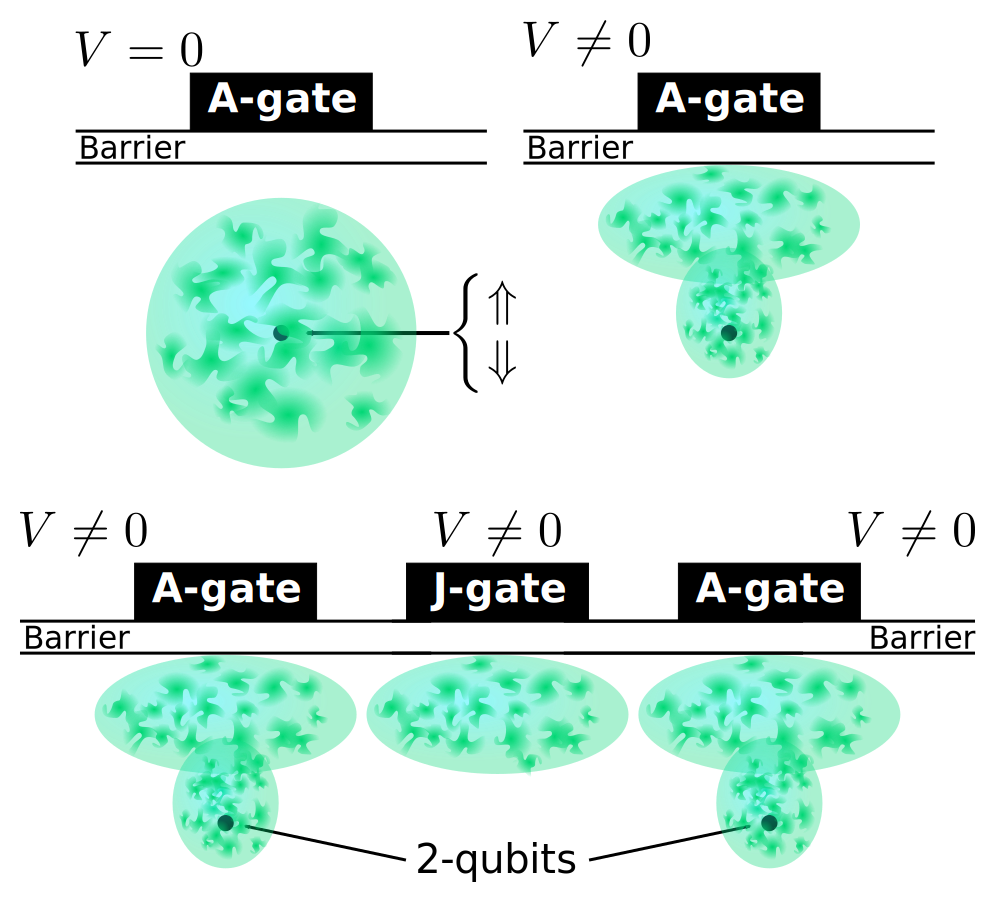
\includegraphics{chapter03/figures/kane.pdf}
\vspace{-5pt}
\caption{Artistic depiction of the Kane proposal for a quantum computer. The single qubit operations would be performed modifying the electronic spin and tunning the hyperfine coupling (witha an electric gate $A$) to interact with the nuclear spin. The two qubit operations would be performed by an electronic mediated state controlled also with an intermediate electric gate $J$.}
\label{kane}
\end{figure}
\FloatBarrier
%~~~~~~~~~~~~~~~~~~~~~~~~~~~~~~~~~~~~~~~~~~~~~~~~~~~~~~~~~~~%
Similarly for two qubits to interact with each other Kane proposed an intermediate gate $J$ to aid the process by increasing (decreasing) the electronic density in between the two qubits.

\section{Morello's Implementation}
Kane proposal has been widely pursued and impresive achievements have been done
\red{Comment on the feasability of this approach. Electron as another qubit? 2-Qubit operations}



\section{The 1-Qubit Hamiltonian}
For the Kane's proposal the description of one qubit is that of a nuclear and an electronic spin in an external magnetic field. We will analyze now the properties of this system.

\subsection{The Zeeman Effect}
The Hamiltonian for a particle with magnetic moment $\vec{m}$ in an external magnetic field $\vec{B}$ is the following:
\begin{equation}
  H_{zee} = -\vec{m}\vec{B}
\end{equation}
The magnetic moment for a particle with mass $m$ and charge $q$ is defined as:
\begin{equation*}
  \vec{m} = g\frac{q}{2m}\vec{S} \qquad\text{with}\quad \vec{S} =
  \frac{\hbar}{2}\vec{\sigma}
\end{equation*}
Where renaming $\mu = \frac{q\hbar}{2m}$ we can express the magnetic moment as:
\begin{equation}
  \vec{m} = g\mu\frac{1}{2}\vec{\sigma}
\label{magmom}
\end{equation}
where $g$ is the so-called g-factor\footnote{The g-factor for the electron and proton are: $g_e=-2.0023\dots$ and $g_p=5.5857\dots$} and $\vec{\sigma}$ is a vector with the Pauli matrices as components $\vec{\sigma}= \left(\sigma_x,\sigma_y,\sigma_z\right)$
\begin{equation}
  \sigma_x=\left(\begin{array}{cc}
    0 & 1 \\
    1 & 0
    \end{array}\right)\quad;\quad
  \sigma_y=\left(\begin{array}{cc}
    0 & -i \\
    i & 0
    \end{array}\right)\quad;\quad
  \sigma_x=\left(\begin{array}{cc}
    1 & 0 \\
    0 & -1
    \end{array}\right)
\end{equation}
The Zeeman term, then, can be rewritten as:
\begin{equation}
  H_{zee} = -\vec{m}\vec{B} = -g\mu\frac{1}{2}\vec{B}\vec{\sigma}
\end{equation}
With an off-plane magnetic field, $\vec{B}=(0,0,B/2)$, this system presents two eigenstates, that we can denote:
\begin{equation}
  \begin{split}
    E_0 &= g\mu\frac{1}{4}B \quad\quad;\quad\quad
    v_0 = \left[\begin{array}{c}
    1\\
    0
    \end{array}\right] = \ket{\uaw}\\
    E_1 &= -g\mu\frac{1}{4}B \quad\quad;\quad\quad
    v_1 = \left[\begin{array}{c}
    0\\
    1
  \end{array}\right] = \ket{\daw}
  \end{split}
\end{equation}
Notice that if we start in any of the eigenstates we can modify the wave function to achieve any generic state $\ket{\psi} = \alpha\ket{\uaw}+\beta\ket{\daw}$ with $\alpha^2+\beta^2 = 1$ simply by applying the appropriate in-plane magnetic field during the appropriate time.\\


Since we would have a nuclear spin \textbf{and} an electronic spin, we would have the corresponding term for each one of them.
\begin{equation}
  H_{zee} = -g_e\mu_e\frac{1}{2}\vec{B}\vec{\sigma}^e - g_p\mu_p\frac{1}{2}\vec{B}\vec{\sigma}^p
\end{equation}

For each of these terms (considered independently) the associated splitting would be of the following order:
\begin{equation}
  \begin{split}
    \Delta_e = g_e\mu_e\frac{1}{2} &\simeq \SI{58}{\micro\eV\per\tesla} \\  %58 \mu eV/T \\
    \Delta_p = g_p\mu_p\frac{1}{2} &\simeq \SI{8.8e-2}{\micro\eV\per\tesla}
    % 8.8\cdot10^{-2}\mu eV/T
  \end{split}
\end{equation}
Since $g_p\simeq g_e/2000$ the nuclear splitting is expected to be around 3 orders of magnitude smaller than the electronic splitting.



\subsection{Hyperfine Interaction}
\label{sec:hyperfine}
Apart from the interaction of the electron and the proton with the external magnetic field we have to take into account the interaction between them.

The hyperfine (HF) interaction arises when we consider the effect of the nuclear spin on the electron.

By introducing the potential vector $\vec{A}_{I}$ (corresponding to the magnetic field created by the proton, $\rotac{\vec{A}_{I}}$) in the Hamiltonian and expanding to first order in this potential vector, we get the complete hyperfine Hamiltonian
\begin{equation}
H_{hf} = \frac{-\mu_{0}}{4\pi}\left[
\frac{q_{p}}{m_{e}R^{3}}\vec{L}\cdot\vec{M}_{I} +
\frac{1}{R^{3}}\left(3(\vec{m}_{e}\cdot\hat{n})
                      (\vec{m}_{p}\cdot\hat{n})-
                      \vec{m}_{e}\cdot\vec{m}_{p}\right) +
\frac{8\pi}{3}\vec{m}_{e}\cdot\vec{m}_{p}\delta(\vec{R})
\right]
\label{full_HF}
\end{equation}
where $\vec{L}$ is the orbital momentum of the electron, $\vec{m}_{e}$ is the spin magnetic moment of the electron, and $\hat{n}$ is the unit vector of the straight line joining the proton to the electron.\\

The first term in equation \eqref{full_HF} represents the interaction of the nuclear magnetic moment with the magnetic field created at the proton by the rotation of the electronic charge. If we are considering $s$ orbitals this term will vanish since all the terms would include a factor like $\bra{n,0,0}L\ket{n,0,0} = 0$, so we will drop this term from the discussion.

The second term represents the dipole-dipole interaction between the nuclear and electronic magnetic moments. Again for a \textit{pure} $s$ orbital this term would vanish as a consequence of the spherical symmetry of the orbital. Nevertheless, because of perturbations (from the crystal or external fields) a contribution from this term may become relevant. \red{review}

The third term is the so-called ``contact term'', and arises from the singularity at $\vec{R}=\vec{0}$ of the field created by the magnetic moment of the proton.
This contact term describes the interaction of the magnetic moment of the electron spin with the the magnetic field inside the proton (considered as punctual). Notice that because of the presence of the delta function in this term, it will be proportional to the overlap of the wave function of the electron and the proton. This term will by the main contribution to the hyperfine interaction.\\

For the case of free, isolated Hydrogen and for the $1s$ orbital the calculation of the contact term can be done exactly:
\begin{equation}
H^{contact}_{hf} =
%\underbrace{\frac{-\mu_{0}}{4\pi}\frac{8\pi}{3}\frac{g_{p}\mu_{n}}{\hbar}
%\frac{g_{e}\mu_{e}}{\hbar}}_{\mathcal{A}_{0}} \vec{I}\vec{S}
\frac{-2\mu_0}{3}\frac{g_{p}\mu_{n}}{2}
\frac{g_{e}\mu_{e}}{2} \bra{1,0,0}\delta(\vec{R})
\ket{1,0,0}  \vec{\sigma}_e\vec{\sigma}_p =
\mathcal{A}_{0}\vec{\sigma}_e\vec{\sigma}_p
\end{equation}
where the notation for the kets is $\ket{n,l,m_{l}}$, and the hyperfine
coupling, $\mathcal{A}_{0}$, takes the value \red{(Units done in the last appendix, check)}: %XXX
\begin{equation}
\frac{\mathcal{A}_{0}\hbar}{2\pi} \simeq 1420 \text{MHz}
\end{equation}
%XXX
correct?:
\begin{equation}
\frac{4\pi\mathcal{A}_{0}}{\hbar} \simeq 1420 \text{MHz?}
\end{equation}

Notice that the contribution to the hyperfine contact term for $p$ (or higher $l$) orbitals vanishes since the wave function vanishes at the nucleus position, and then, the factor $\bra{n,l,m_{l}}\delta(\vec{R})\ket{n,l,m_{l}}$ will always be zero.\\

In general the effective hyperfine coupling of a given state will be considered proportional to the weight of the wave function on the Hydrogen $s$ orbital.

\begin{equation}
  \mathcal{A} = A_0|\braket{\phi_s}{\psi}|^2
\end{equation}

Of course other orbitals centered at the other atoms would also contribute to the hyperfine interaction (since the wave function does not vanish at the position of the nucleus), nevertheless the \ac{tb} approximation does not offer the tools to deal with the deformation of the orbitals what makes it impossible to estimate the evaluation of the orbitals at the $H$ nucleus.

For the case of Si:$^{31}$P the hyperfine coupling in MegaHertz is $4\pi\mathcal{A}/\hbar=58MHz$
\red{check factor}


\subsection{The full 1-qubit Hamiltonian}
Finally, we can write the complete Hamiltonian for our nuclear qubit as a combination of the previous ones:
\begin{equation}
  H = -g_e\mu_e\frac{1}{2}\vec{B}\vec{\sigma}^e
      -g_p\mu_p\frac{1}{2}\vec{B}\vec{\sigma}^p
      +A\vec{\sigma}^e\cdot\vec{\sigma}^p
\label{1qubit}
\end{equation}
First of all, we can make a quick estimation of the order of magnitude of each of these terms:
\begin{itemize}
  \item Zeeman for the electron: $g_e\mu_e\simeq\SI{-115.9}{\micro\eV\per\tesla}$
  % -2\cdot5.79\cdot10^{-5}\simeq-1.16\cdot10^{-4}eV/T$
  \item Zeeman for the proton: $g_p\mu_p\simeq\SI{0.176}{\micro\eV\per\tesla}$
  % 5.6\cdot3.15\cdot10^{-8}\simeq1.7\cdot10^{-7}eV/T$
  \item Hyperfine: Assuming
  $\mathcal{A}=58MHz\Rightarrow\mathcal{A}\simeq\SI{0.003}{\micro\eV}$
% 6.6\cdot10^{-08}eV$
\end{itemize}
We are stretching a bit the notation in the Hamiltonian \eqref{1qubit} since each of the terms is expressed in a different basis. Namely, each of the Zeeman terms act only in the electron \textbf{or} proton spin subspace but the hyperfine coupling has to be expressed in a 2-particle basis that have not defined yet.
To fix the notation we define the following 2-particle basis:
\begin{equation}
  \mathcal{B}=\left\{\ket{\uaw\Uaw},\ket{\uaw\Daw},
                     \ket{\daw\Uaw},\ket{\daw\Daw}\right\}
\label{basis}
\end{equation}
where the simple arrows $\uaw\daw$ represent the $S_z$ eigenvectors of the electronic spin, and the double arrows $\Uaw\Daw$ represent the $S_z$ eigenvectors of the nuclear spin.

In this basis the Pauli matrices are expressed as follows.
\begin{equation}
  \begin{split}
    \sigma^e_x=\left(\begin{array}{cccc}
    0 & 0 & 1 & 0 \\
    0 & 0 & 0 & 1 \\
    1 & 0 & 0 & 0 \\
    0 & 1 & 0 & 0
    \end{array}\right)\quad;\quad
    \sigma^e_y=\left(\begin{array}{cccc}
    0 & 0 & -i & 0 \\
    0 & 0 & 0 & -i \\
    i & 0 & 0 & 0 \\
    0 & i & 0 & 0
    \end{array}\right)\quad;\quad
    \sigma^e_z=\left(\begin{array}{cccc}
    1 & 0 & 0 & 0 \\
    0 & 1 & 0 & 0 \\
    0 & 0 & -1 & 0 \\
    0 & 0 & 0 & -1
    \end{array}\right)\\
    \sigma^p_x=\left(\begin{array}{cccc}
    0 & 1 & 0 & 0 \\
    1 & 0 & 0 & 0 \\
    0 & 0 & 0 & 1 \\
    0 & 0 & 1 & 0
    \end{array}\right)\quad;\quad
    \sigma^p_y=\left(\begin{array}{cccc}
    0 & -i & 0 & 0 \\
    i & 0 & 0 & 0 \\
    0 & 0 & 0 & -i \\
    0 & 0 & i & 0
    \end{array}\right)\quad;\quad
    \sigma^e_z=\left(\begin{array}{cccc}
    1 & 0 & 0 & 0 \\
    0 & -1 & 0 & 0 \\
    0 & 0 & 1 & 0 \\
    0 & 0 & 0 & -1
    \end{array}\right)
  \end{split}
\end{equation}
Hence, our Hamiltonian for two qubits in the presence of an off-plane magnetic field, $\vec{B}=(0,0,B/2)$, can be expressed as follows:
\begin{equation*}
H = \underbrace{-g_e\mu_e\frac{1}{4}}_{E}B\sigma^e_z
    \underbrace{-g_p\mu_p\frac{1}{4}}_{P}B\sigma^p_z
    +A\vec{\sigma}^e\cdot\vec{\sigma}^p
\end{equation*}
\begin{equation}
  H = \left(\begin{array}{cccc}
  B(E+P)+A & 0 & 0 & 0 \\
  0 & B(E-P)-A & 2A & 0 \\
  0 & 2A & B(-E+P)+A & 0 \\
  0 & 0 & 0 & B(-E-P)-A
  \end{array}\right)
\end{equation}

The eigenvalues of this matrix are the following \red{irrelevant?}:
\begin{equation}
  \begin{split}
    E_0 &= -A-B(P+E) \quad;\quad v_0=\left(0,0,0,1\right)\\
    E_1 &= A+B(P+E) \quad;\quad v_1=\left(1,0,0,0\right)\\
    E_2 &= -\sqrt{A(5A+2B(P-E)) + B^2 (P-E)^2} \\
        &\quad\quad\quad\quad v_2 =\left(0,-\frac{A+B(P-E)+\sqrt{A(5A+2B(P-E)) + B^2 (P-E)^2}}{2 A},1,0\right)\\
    \quad\\
    E_3 &= \sqrt{A(5A+2B(P-E)) + B^2 (P-E)^2}\\
        &\quad\quad\quad\quad v_3 = \left(0,-\frac{A+B(P-E)-\sqrt{A(5A+2B(P-E)) + B^2 (P-E)^2}}{2 A},1,0\right)
  \end{split}
\label{eig}
\end{equation}



For now we will neglect the contribution of the proton and check the behavior of the eigenenergies of the system as a function of both the external magnetic field and the hyperfine coupling.
%~~~~~~~~~~~~~~~~~~~~~~~~~~ FIGURE ~~~~~~~~~~~~~~~~~~~~~~~~~%
\begin{figure}[h!]
\centering
\includegraphics[width=0.9\textwidth]{chapter03/figures/spectrum.png}
\vspace{-5pt}
\caption{Evolution of the eigenvalues of the Hamiltonian \eqref{1qubit} with the magnetic field, $B$, and the hyperfine interaction, $\mathcal{A}$. The dashed line is used to indicate the magnetic field in the second figure}
\label{spectrum}
\end{figure}
\FloatBarrier
%~~~~~~~~~~~~~~~~~~~~~~~~~~~~~~~~~~~~~~~~~~~~~~~~~~~~~~~~~~~%
In figure~\ref{spectrum} we can see that the energy levels are separated in two sets split by the electronic Zeeman splitting (remember that we are neglecting the proton Zeeman coupling here). The splitting within each of these sets is governed by the hyperfine coupling.

But as we said before, the hyperfine coupling and Zeeman coupling for the proton are in the same order of magnitude. When we include the proton Zeeman interaction the big picture is the same: two set of levels split by the electronic Zeeman. But within each of these two sets there is a difference, depending on the magnitude of the magnetic field and the hyperfine coupling the ordering of the wave functions may change. \red{rephrase}
%~~~~~~~~~~~~~~~~~~~~~~~~~~ FIGURE ~~~~~~~~~~~~~~~~~~~~~~~~~%
\begin{figure}[h!]
\centering
\includegraphics[width=0.9\textwidth]{chapter03/figures/pro_nopro.png}
\vspace{-5pt}
\renewcommand{\figurename}{\footnotesize{\textsc{Figure}}}
\caption{Comparison of the energy levels as a function of the hyperfine coupling. Panel $a)$ neglects the Zeeman term for the proton, in panel $b)$ we use the full Hamiltonian. (Both panels share the $Y$ axis)}
\label{proton}
\end{figure}
\FloatBarrier
%~~~~~~~~~~~~~~~~~~~~~~~~~~~~~~~~~~~~~~~~~~~~~~~~~~~~~~~~~~~%
The level crossing that appears in figure~\ref{proton} represents nothing more than the exchange of the wave functions as it can be seen in the analytical expression~\eqref{eig}. In fact using these expressions we can get the expression for this level crossing:
\begin{equation}
  \mathcal{A}_{\times}=\frac{B}{2}\left(E\pm\sqrt{E^2+4EP}\right)
\end{equation}


To clarify the meaning of this spectrum we make a schematic representation of the eigenfunctions, shown in figure~\ref{levels1Qbit}. The left column in the table represents the wave functions neglecting the proton's Zeeman contribution. The two columns in the right do not neglect the proton's coupling, and show the cases of high magnetic field (or low hyperfine coupling) and low magnetic field (or high hyperfine coupling). It is clear that depending on the relative magnitude of the proton's Zeeman effect and the Hyperfine coupling the order of the wave functions may differ.
%~~~~~~~~~~~~~~~~~~~~~~~~~~ FIGURE ~~~~~~~~~~~~~~~~~~~~~~~~~%
\begin{figure}[h!]
\centering
\includegraphics{chapter03/figures/levels1Qbit.pdf} %levels.png}
\vspace{-5pt}
\caption{Sketch of the energy levels for the 1 Qubit hamiltonian~\eqref{1qubit}. The splitting among the different states is mainly due to the electronic Zeeman terms. The lowest energy state is determined by the competition between the nuclear Zeeman splitting and the hyperfine interaction.}
% \caption{Schematic representation of the energy levels and its respective wave functions. The states $\ket{\daw\Uaw}$ and $\ket{\uaw\Daw}$ and in fact mixed, but it is negligible (this means that $\ket{\uaw\Daw}\simeq0.9999999\ket{\uaw\Daw}+0.0002672\ket{\daw\Uaw}$). All the possible transitions are specified by $\delta_i$.}
\label{levels1Qbit}
\end{figure}
\FloatBarrier
%~~~~~~~~~~~~~~~~~~~~~~~~~~~~~~~~~~~~~~~~~~~~~~~~~~~~~~~~~~~%
The states $\ket{\daw\Uaw}$ and $\ket{\uaw\Daw}$ do not in fact appear with weight 1, instead there is a small mixing (less than $0.001\%$).

\red{I think the order of my states is not exactly the same as Morello's. Check}
Notice that $\delta_1$ and $\delta_2$ will be quite similar ($\SI{50}{\eV/\tesla}$) and $\delta_3$, $\delta_4$ will also be very similar ($\SI{0.05}{\eV/\tesla}$). These frequencies correspond to the energy necessary for flipping respectively the electron spin and the nuclear spin.

\red{Nuclear magnetic resonance and stuff}


\section{The 2-Qubit Hamiltonian}
The general expression for the Hamiltonian for two qubits requires the consideration of Zeeman interactions for each of the electronic and nuclear spins, hyperfine coupling for each of the qubits, and an exchange term. Of course contributions such as  $\mathcal{A}_{1,2}\vec{\sigma}^e_1\vec{\sigma}^e_2$ should also exist, but its contribution would be negligible since the electronic wavefunction decays exponentially. The total Hamiltonian for two qubits, then, reads:
\begin{equation}
  H = H_B +A_1\vec{\sigma}^e_1\cdot\vec{\sigma}^p_1
      +A_2\vec{\sigma}^e_2\cdot\vec{\sigma}^p_2
      +J\vec{\sigma}^e_1\cdot\vec{\sigma}^e_2
\label{ham2Q}
\end{equation}
where $H_B$ contains the Zeeman interactions of each of the electronic and nuclear spins.
\begin{equation}
  H_B = -g_e\mu_e\frac{1}{2}\vec{B}_1\vec{\sigma}^e_1
      -g_p\mu_p\frac{1}{2}\vec{B}_1\vec{\sigma}^p_1
      -g_e\mu_e\frac{1}{2}\vec{B}_2\vec{\sigma}^e_2
      -g_p\mu_p\frac{1}{2}\vec{B}_2\vec{\sigma}^p_2
\label{ham2Q_zeeman}
\end{equation}
To describe two qubits we need again to expand our basis. In particular we will use the notation $\ket{S^z_1I^z_1;S^z_2I^z_2}$. The basis, then, would have 16 elements
\begin{equation}
\begin{split}
 \mathcal{B}_{2Q} =  \left\{\ket{\uaw\Uaw;\uaw\Uaw},\ket{\uaw\Uaw;\uaw\Daw},\ket{\uaw\Uaw;\daw\Uaw},\ket{\uaw\Uaw;\daw\Daw},\right.\\
        \ket{\uaw\Daw;\uaw\Uaw},\ket{\uaw\Daw;\uaw\Daw},\ket{\uaw\Daw;\daw\Uaw},\ket{\uaw\Daw;\daw\Daw},\\
        \ket{\daw\Uaw;\uaw\Uaw},\ket{\daw\Uaw;\uaw\Daw},\ket{\daw\Uaw;\daw\Uaw},\ket{\daw\Uaw;\daw\Daw},\\
 \left.\ket{\daw\Daw;\uaw\Uaw},\ket{\daw\Daw;\uaw\Daw},\ket{\daw\Daw;\daw\Uaw},\ket{\daw\Daw;\daw\Daw} \right\}
\end{split}
\end{equation}
Notice that we are not considering here doubly occupied states such as $\ket{\udaw\Uaw;\quad\Uaw}$ since for now we consider that the two qubits are sufficiently isolated from each other to allow this kind of transitions, in addition to the extra energy that would cost the double occupancy (Hubbard repulsion).

All the operators in eq.~\eqref{ham2Q} have the same dimension as the basis ($16\times16$) and, when diagonalized, they show a spectrum similar to that sketched in fig.~\ref{levels2Qbits}
%~~~~~~~~~~~~~~~~~~~~~~~~~~ FIGURE ~~~~~~~~~~~~~~~~~~~~~~~~~%
\begin{figure}[h!]
\centering
  \includegraphics{chapter03/figures/levels2Qbits.pdf}
\vspace{-5pt}
\caption{Sketch of the energy levels of 2 qubits. The spectrum is divided in three sets of levels determined mainly by the electronic Zeeman splitting. The degeneracies and ordering of the states in each of these groups is determined by competition between the nuclear Zeeman and hyperfine couplings as well as the exchange interaction.}
\label{levels2Qbits}
\end{figure}
\FloatBarrier
%~~~~~~~~~~~~~~~~~~~~~~~~~~~~~~~~~~~~~~~~~~~~~~~~~~~~~~~~~~~%
As we  can see the  levels are split in three sets. The energy of each of these sets is mainly defined by the electronic spin of the two qubits, eq.~\eqref{ham2Q_zeeman} since that is the strongest interaction.
When the electrons of each of the Qubits are parallel (both up or down) the total energy of the system is roughly $E=pm g_e\mu_e B$.
The competition between the Zeeman effect in the nuclear spin and the hyperfine coupling determines which state is the lowest in energy, either $\ket{\Uaw;\Uaw}$ or $\ket{\Daw;\Daw}$. Notice that the solutions in which both electronic spins are parallel and the nuclear spin in each Qubit are different are degenerate in energy.


\section{The Graphene analogue}
In hydrogenated graphene we have very similar objects. The Hydrogen has a single nuclear spin, the proton, and the electronic states around it would provide the other spin.

The electronic properties of graphene are highly tunable what suggest that maybe the interactions are tunable as well.

Also the $C$ atoms provide almost no nuclear spins (the abundance of $^{12}C$ is about $98.9\%$ while $^{13}C$ is about $1.1\%$ and only negligible traces of other isotopes~\cite{iupac}), so long relaxation times for the nuclear spin is to be expected


\red{Explain here the similarities and general idea. Possible advantages and drawbacks.}
\red{Motivation for studying graphene and hydrogenated graphene.}


%~~~~~~~~ Chapter ~~~~~~~~
% Graphene
\chapter{Graphene}
\label{ch:graphene}
Graphene is one of the most studied materials ever. It consists of a two-dimensional array of $C$ atoms arranged in a honeycomb lattice like that of the Fig.~\ref{graphene_structure}~($a-d$). The honeycomb lattice is not a Bravais lattice so in order to describe such a system (in terms of Bloch functions) we can choose a wide variety of unit cells and lattice vectors. The simplest choice is the two atoms unit cell with a triangular Bravais lattice as shown in Fig~\ref{graphene_structure}~(a). Nevertheless any other choice of unit cell and lattice vectors is valid as long as it tessellates the space. %XXX
%~~~~~~~~~~~~~~~~~~~~~~~~~~ FIGURE ~~~~~~~~~~~~~~~~~~~~~~~~~%
\begin{figure}[h!]
\centering
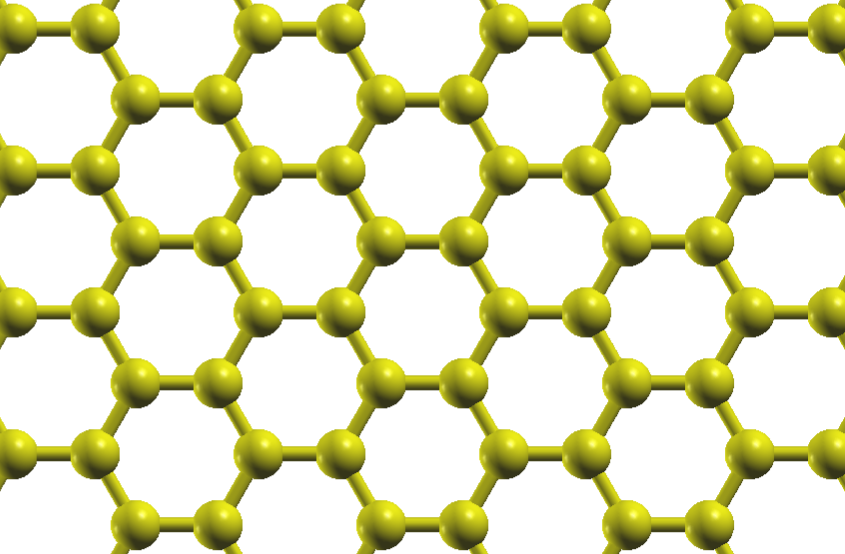
\includegraphics[width=\textwidth]{chapter04/figures/graphene.pdf}
\vspace{-5pt}
\caption{$(a-d)$ Graphene atomic structure considering differnt unit cells and lattice vectors. $(e)$ relevant hydrogenic orbitals for the $C$ atom.}
\label{graphene_structure}
\end{figure}
\FloatBarrier
%~~~~~~~~~~~~~~~~~~~~~~~~~~~~~~~~~~~~~~~~~~~~~~~~~~~~~~~~~~~%
Carbon atoms have 6 \ac{el}, 2 in the 1s level, 2 more in the 2s level and finally another 2 \ac{el} in the 2p level. Since the orbitals $n=1$ are full and very far in energy there is no need to consider them.
The 2s level is also full, but not so far from the Fermi energy, so we will take a look at its importance.
We will study the 2p orbitals in two groups since the $p_z$ orbital has no hopping to the other $p$ orbitals due to mirror symmetry (Fig.~\ref{graphene_structure}~(e)).
%TODO



\section{Slater-Koster tight-binding model}
\label{sec:SK}
Generally the hopping parameters are an input in any \ac{tb} model, and usually they are calculated by fitting eigenvalues and eigenfunctions obtained from \ac{dft} calculations (the eigenfunctions are usually projected to a basis of localized atomic orbitals) or by fitting experimental data.

As a system grows complex, more and more parameters are needed to describe it, nevertheless since the number of different orbitals is finite, one could expect that not all the parameters are completely independent from the others.


The \ac{sk} approximation takes into account the symmetry of the orbitals to reduce the number of parameters needed. Due to the symmetry of the atomic orbitals it is to be expected that different hoppings could be related. It is easier to see this point with an example.
%~~~~~~~~~~~~~~~~~~~~~~~~~~ FIGURE ~~~~~~~~~~~~~~~~~~~~~~~~~%
\begin{figure}[h!]
\centering
\includegraphics{chapter04/figures/complex.png}
\vspace{-5pt}
\caption{Relation between $t_{p_{z},p_{x}}$ and $t_{p_{z},p_{y}}$ hopping. In this case we need not only to rotate each orbital but also the position of the atoms, but it is clear that one hopping can be calculated from the other.}
\label{complex}
\end{figure}
\FloatBarrier
%~~~~~~~~~~~~~~~~~~~~~~~~~~~~~~~~~~~~~~~~~~~~~~~~~~~~~~~~~~~%
In figure~\ref{complex} we can see that the hoppings $t_{p_{z},p_{x}}$ and $t_{p_{z},p_{y}}$ are in fact related by a rotation of the system, and we could expect that they would be functionally equal.
If we define the unitary vector $\hat{r} = \vec{r}/|\vec{r}|$ and call its components $l$, $m$, $n$, ($\hat{r}=(l,m,n)$) we can see that
\begin{equation}
  t_{p_{z},p_{x}} (l,m,n) = t_{p_{z},p_{y}}(m,l,n)
\end{equation}
notice that the change in the arguments is equivalent to perform a rotation of the vector $\vec{r}$ of $-\pi/2$ around the $Z$ axis, as shown in Fig.~\ref{complex}.

By doing this kind of transformations we can see that all the ($p-p$) hoppings can be decomposed in just two kinds of bonds depending on the relative orientation of the orbitals. This is illustrated in figure~\ref{bonds}.
%~~~~~~~~~~~~~~~~~~~~~~~~~~ FIGURE ~~~~~~~~~~~~~~~~~~~~~~~~~%
\begin{figure}[h!]
\centering
\includegraphics{chapter04/figures/bonds.png}
\vspace{-5pt}
\caption{$a)$ Only two different types of bonds between $p$ orbitals. $b)$ Simplification of the \ac{sk} hopping parameter by decomposing the hopping into its $\sigma$ and $\pi$ component, in this case it is easy to see that the hopping from any $p_{z}$ orbital to another one that in the $XY$ plane will be purely a $\pi$ bond.}
\label{bonds}
\end{figure}
\FloatBarrier
%~~~~~~~~~~~~~~~~~~~~~~~~~~~~~~~~~~~~~~~~~~~~~~~~~~~~~~~~~~~%
We can notice that in the case of graphene, where close to the Fermi energy the only involved orbitals are $p_{z}$ and, since all the hoppings are in-plane ($n=0$), all the bonds will be purely $\pi$ bonds, just because of the symmetry of the orbitals.\\


In the \ac{sk} approximation the atomic distances are encoded in the magnitude of the bonds, $V_{ss\sigma}$, $V_{sp\sigma}$, $V_{pp\sigma}$, $V_{pp\pi}$ (we will call them simply \ac{sk} parameters for short). The coefficients ($l$, $m$, $n$) in the analytic formulas are the responsible for capturing the symmetries arising both form the orbital (sign) and from the atomic structure (direction).\\

This decoupling of magnitude and direction in the hoppings provides a simple model able to capture the effects of geometric deformations, and any symmetry (breaking) in the atomic structure. For instance the effect of buckling in graphene is easily captured by this model.\blue{bands, bands with buckling,...}

\red{explain better}
The effect due to a reduction/increase of the hopping would be included by modifying the \ac{sk} parameters, yet the dependence of this parameters with the interatomic distance is not always easy to calculate.\\

At the end of the day the \ac{sk} approximation results in a reduction of the parameters needed to describe the hoppings in the system. For example, in a system with $s$, $p_x$, $p_y$, $p_z$, $d_{xy}$, $d_{yz}$, $d_{zx}$, $d_{x^{2}-y^{2}}$ and $d_{3z^{2}-r^{2}}$ we would expect 36 parameters to describe all the different hoppings, but within the \ac{sk} approximation we would only need 10 parameters.\\


The main drawback for the \ac{sk} model is to actually obtain the \ac{sk} parameters. In fact it is not guaranteed (at all) that for any given system a set of \ac{sk} parameters should exist.
Knowing that this approximation is based upon the symmetry of the atomic orbitals it is expected that for systems where the atomic orbitals are heavily hybridized this description will not suffice.

\red{Discussion limits, covalent, deformation, localized orbitals}



\section{Physical properties of Graphene}
\subsection{Bands}
Here some bands with Slater-Koster, maybe include bismuth, BN, Zeeman, SOC...
%~~~~~~~~~~~~~~~~~~~~~~~~~~ FIGURE ~~~~~~~~~~~~~~~~~~~~~~~~~%
\begin{figure}[h!]
\centering
\includegraphics{chapter04/figures/graphene_bands.png}
\vspace{-5pt}
\caption{Graphene bands in the \ac{sk} approximation, with $s$, $p_x$, $p_y$, $p_z$ orbitals for the $C$ atoms. The color denote the $p_z$ component of each state. It can be seen that the $p_z$ orbital are decoupled from the rest of the orbitals and at low energy they are enough to describe the system}
\label{Gbands}
\end{figure}
\FloatBarrier
%~~~~~~~~~~~~~~~~~~~~~~~~~~~~~~~~~~~~~~~~~~~~~~~~~~~~~~~~~~~%

\subsection{Quantum Spin Hall}
\ac{qsh} in multilayers


%~~~~~~~~ Chapter ~~~~~~~~
% Graphene Bilayer
\chapter{Graphene Bilayer}
\section{Introduction}
When $N$ vacancies are introduced, $N$ in-gap states appear. If we consider only one orbital per site, then all the states appear at $E=0$ as dictated by the Lieb's theorem (bipartite lattice at half filling in the limit of $U\to 0$).

When an electric field is applied to graphene bilayer (GBL) a gap is opened at the Dirac points. For reasonable electric fields, the gap opens linearly with the electric field, until at some point it saturates. The maximum experimentally observed value of the gap is\cite{Zhang2009} $\Delta=250meV$.

We are going to consider a 0D system, a hexagonal island with armchair edges. It contains over 90000 atoms (91812, to be precise) and the bilayer is stalked in a Bernal way.
The electric field is introduced as an energy imbalance between the two graphene layers, and the vacancies are considered as an infinite on-site energy. For now we will just consider that the vacancies are placed along the $X$ axis (namely, $\alpha=0$).

Since we consider a 0D system, no bands can be defined, hence only the spectrum can be calculated. Since the full diagonalization of such a system would be almost impossible (for an average computer) we will take advantage of the Lanczos diagonalization method\cite{Arnoldi1951,Lanczos1950}, already available in a number of standard libraries.
This computation method provides the $n$ eigenstates closest to a given energy, in our case we will consider a few more eigenstates than in-gap states should appear in order to be sure that the conduction and valence states are also captured.

For a given electric field, the result of our calculation is just the spectrum: a set of eigenenergies and eigenvectors. When we repeat the calculation for different electric fields we can see the smooth variation of the states as a function of the electric field.

\section{Two vacancies}
The typical evolution of the spectrum of an island with 2 vacancies is shown in Fig.~\ref{2vacs}. For a given


%~~~~~~~~ Chapter ~~~~~~~~
% A Graphene based Quantum Computer
\chapter{Hydrogenated Graphene Bilayer}
\label{ch:bilayer}
Kane's proposal~\cite{Kane1988}, and all the experimental realizations of it~\cite{Morello2010}, based the control of the Qubits in the manipulation of the electronic states with an electric gate that would modify the electronic cloud around the $^{31}P$ nucleus.

Since graphene is a purely \ac{2dm} its electronic properties are highly tunable by proximity, electric gating or other techniques. First we make a quick review of the properties of \ac{gb} and the effect of an external electric field and then we explore the possibility of the realization of 1 and 2-Qubit operations.

\section{Graphene Bilayer}
The minimal unit cell for describing a \ac{gb} contains four atoms, disposed as seen in the inset in Fig.~\ref{bilayer}. The lattice vectors describing the Bravais lattice are the same as in the case of monolayer graphene. Since the interlayer distance, around $d \sim \SI{3.0}{\angstrom}$, is  around three times bigger than the C-C distance\footnote{around $d_{C-C} = \SI{1.4}{\angstrom}$}, it is expected that the interlayer hopping will be smaller, in fact from literature~\cite{KatsnelsonBook} we get that the interlayer hopping $t'\simeq 0.15t_{\pi-\pi}\simeq\SI{0.4}{\eV}$. The effect of the interlayer interaction is to ``parabolize'' the linear bands around the $K$ points and double the $p_z$ manifold bands.
%~~~~~~~~~~~~~~~~~~~~~~~~~~ FIGURE ~~~~~~~~~~~~~~~~~~~~~~~~~%
\begin{figure}[h!]
\centering
\includegraphics{chapter06/figures/bilayer_bandDOS.pdf}
\vspace{-5pt}
\caption{Band structure and \ac{dos} of bilayer graphene. The red shadowed region shows the contribution of the $p_z$ manifold.}
\label{bilayer}
\end{figure}
\FloatBarrier
%~~~~~~~~~~~~~~~~~~~~~~~~~~~~~~~~~~~~~~~~~~~~~~~~~~~~~~~~~~~%
The $p_z$ bands at the $K$ point are split by an amount proportional to the interlayer hopping

Notice that in the bilayer the $p_z$ manifold is no longer decoupled from the rest of the orbitals (for instance there is a finite hopping between $p_z$ orbitals from one layer and $s$ orbitals of the other), nevertheless close to the Fermi energy the approximation of considering only $p_z$ orbitals is still justified.
The general aspect of the \ac{dos} is similar to that of the graphene but it is important to notice that at $E=0$ the \ac{dos} is now finite.

 \section{Effect of the electric field}
The main effect of an external electric field applied to bilayer graphene is to shift the (on-site) energy of the electrons, we can write such a Hamiltonian term like

\begin{equation}
  H_{\vec{E}} = \lambda_{\vec{E}}\sum_i \varepsilon_l \crea{c}{i}\des{c}{i}
\end{equation}
where $\varepsilon_l=\pm1$ depending on the layer, $l$,  of the atom $i$.
The effect of such a term in \ac{gb} is just to open a gap~\cite{Yamashiro2012} close to the Fermi energy as shown in fig~\ref{bi_Efield}.

%~~~~~~~~~~~~~~~~~~~~~~~~~~ FIGURE ~~~~~~~~~~~~~~~~~~~~~~~~~%
\begin{figure}[h!]
  \centering
  \includegraphics[width=\textwidth]{chapter06/figures/bilayer_elec.pdf}
  \vspace{-10pt}
  \caption{\ac{dos} of a bilayer graphene system in the absence (left panel) and presence (right panel) of an electric field $E=\SI{0.5}{\eV}$.} %XXX UNITS
  \label{bi_Efield}
\end{figure}
\FloatBarrier
%~~~~~~~~~~~~~~~~~~~~~~~~~~~~~~~~~~~~~~~~~~~~~~~~~~~~~~~~~~~%

% Analogously to the discussed scenario of a vacancy in (monolayer) graphene, the introduction of a vacancy also results in the appearance of a ``zero energy state''. In the presence of an external electric field the impurity state will not appear at $E=0$ but shifted in energy as shown in fig.~\ref{dos_bi_dfct}

% %~~~~~~~~~~~~~~~~~~~~~~~~~~ FIGURE ~~~~~~~~~~~~~~~~~~~~~~~~~%
% \begin{figure}[h!]
% \centering
% \includegraphics{chapter06/figures/bilayer_dos_dfct.png}
% \vspace{-5pt}
% \caption{\ac{dos} of bilayer graphene with (green line) and without (blue line) a vacancy in the presence of an external electric field. The left and right panels have been calculated for electric fields of opposite sign, notice that }
% \label{dos_bi_dfct}
% \end{figure}
% \FloatBarrier
% %~~~~~~~~~~~~~~~~~~~~~~~~~~~~~~~~~~~~~~~~~~~~~~~~~~~~~~~~~~~%

\subsection{About the charge neutrality}
when a bias is applied to \ac{gb} there is the chance that some charge is transferred form one layer to the other\cite{Wang2016a,Zhang2009}. To be sure of how relevant this effect is we calculate where the Fermi Energy lies as well as the charge in each layer.



% % The position where the adatom is introduced now is important since one of the sublattices of each layer is fully connected to the other layer. All the possibilities for the H chemisorption are depicted in figure\red{FIG}. We will consider only the structure (b).
% %
% % %~~~~~~~~~~~~~~~~~~~~~~~~~~ FIGURE ~~~~~~~~~~~~~~~~~~~~~~~~~%
% % \begin{figure}[h!]
% % \centering
% % \includegraphics{chapter06/figures/bilayer_H.pdf}
% % \vspace{-5pt}
% % \caption{All opssible atomic strucutre for chemisorbed H}
% % \end{figure}
% % %~~~~~~~~~~~~~~~~~~~~~~~~~~~~~~~~~~~~~~~~~~~~~~~~~~~~~~~~~~~%
% %
% %
% %
% % \subsection{Electric control of the hyperfine interaction}
% % Electric control of the hyperfine with the bias in the bilayer.
% % %~~~~~~~~~~~~~~~~~~~~~~~~~~ FIGURE ~~~~~~~~~~~~~~~~~~~~~~~~~%
% % \begin{figure}[h!]
% % \centering
% % \includegraphics{chapter06/figures/hyperfine.png}
% % \vspace{-5pt}
% % \caption{Hyperfine dependence with the bias voltage.}
% % \end{figure}
% % \FloatBarrier
% % %~~~~~~~~~~~~~~~~~~~~~~~~~~~~~~~~~~~~~~~~~~~~~~~~~~~~~~~~~~~%
% %
% % A similar behavior can be seen from the gap.
% % %~~~~~~~~~~~~~~~~~~~~~~~~~~ FIGURE ~~~~~~~~~~~~~~~~~~~~~~~~~%
% % \begin{figure}[h!]
% % \centering
% % \includegraphics{chapter06/figures/gap.png}
% % \vspace{-5pt}
% % \caption{Dependence of the gap and the energy of the resonance with the bias voltage.}
% % \end{figure}
% % \FloatBarrier
% % %~~~~~~~~~~~~~~~~~~~~~~~~~~~~~~~~~~~~~~~~~~~~~~~~~~~~~~~~~~~%
% %
% %
\section{1 Hydrogen adatom}
\subsection{General considerations} %~~~~~~~~~~~~~~~~~~~~~~~~~~~~~~~~~~~~~~~~~~%
Everything here is done in an armchair island of bilayer graphene, as such, the system is $0$-D, so there is no translational symmetry and no $\vec{k}$ vector can be defined.

To study these systems we will consider a basis of localized states that could be considered to be the $p_z$ hydrogenoid orbitals.
\begin{equation}
  \mathcal{B} = \left\{\phi_1,\phi_2,\dots,\phi_\beta,\dots,\phi_{N_C}\right\}
\end{equation}

Written in such a basis, the general Hamiltonian and its eigenvectors, then, will look like
\begin{equation}
  H = H_t + H_{\lambda_E} \quad\quad;\quad\quad
  H\ket{\psi_\alpha} = E_\alpha\ket{\psi_\alpha} \quad\quad;\quad\quad
  \ket{\psi_\alpha} = \sum_\beta c_\beta\ket{\phi_\beta}
\label{general}
\end{equation}


The term $H_t$ represents the kinetic energy arising from the hopping between neighboring sites and the term $H_{\lambda_E}$ corresponds to the effect of an external electric field on the electrons. Such a term takes the form:
\begin{equation}
  H_{\lambda_E} = \lambda_E
  \left(\begin{array}{cc}
  \mathds{1} & 0 \\
  0 & -\mathds{1}
  \end{array}\right)
\end{equation}
where the elements $\pm\mathds{1}$ refer to the identity for the upper and lower layer respectively.

The vacancies are introduced in this model as an infinite on-site energy for the chosen atom(s). Unless otherwise stated everything is done in $\si{\eV}$ %$eV$
, \emph{not hopping units}, the $p_z$-$p_z$ hopping is chosen as $t=\SI{-2.7}{\eV}$.





\subsection{Note on the geometry}
Any vacancy considered will always be chosen on a hollow position (see fig~\ref{geo_sketch} $c)$) even if it not specified in the text.

When only one vacancy is considered, it will be placed at the atomic position closest to the center of the island.

When two vacancies are considered they will be placed as separated from the edges as possible, as shown in fig~\ref{geo_sketch} $b)$ since this configuration allows the study of a wider range of the parameters $\alpha$ and $d$. Later in the text another configuration consisting in one vacancy in the center of the island, and the other in different positions $\vec{r}=d\cos(\alpha)+d\sin(\alpha)$.
%~~~~~~~~~~~~~~~~~~~~~~~~~~ FIGURE ~~~~~~~~~~~~~~~~~~~~~~~~~%
\begin{figure}[h!]
\centering
\includegraphics[width=\textwidth]{chapter06/figures/vacs_sketch.pdf}
\vspace{-15pt}
\caption{$a)$ and $b)$ show sketches of the position of the vacancies and relevant geometric information. In the upper left corner the real atomic structure is shown using blue for the lower layer and red for the upper one. The length $L_C$ is the typical size of the in-gap state. $c$ atomic structure showing the ``connected'' and ``hollow'' sites in the upper layer as well as the $A/B$ sublattices (in red/blue).}
\label{geo_sketch}
\end{figure}
\FloatBarrier
%~~~~~~~~~~~~~~~~~~~~~~~~~~~~~~~~~~~~~~~~~~~~~~~~~~~~~~~~~~~%

Note that as long as the border effects are negligible, and due to the $C_3$ symmetry of the in-gap states in graphene, we only need to explore the range of angles between vacancies of $\alpha\in\left[0,60\right]$.


\subsection{Single vacancy} %~~~~~~~~~~~~~~~~~~~~~~~~~~~~~~~~~~~~~~~~~~~~~~~~~~%
Since we are studying an island with a single vacancy, the energy levels are a discrete set of energies. In figure~\ref{1vac_spec} (c) the difference in the spectrum due to the introduction of a vacancy at $\lambda_E=0$ is shown. When a vacancy is introduced, an in-gap state appears at $E=0$ and some \emph{(quasi-)}degeneracies are broken.

The effect of the electric field in the spectrum is shown in figure~\ref{1vac_spec} $a)$ and $b)$. Its main effect is to open a gap, linearly dependent with the electric field.

The shift in the energy at which the in-gap state appears is linear for low electric field, but it remains in-gap for all the regime of electric fields studied. In fig~\ref{1vac_spec} $a$-$c)$ only the eight eigenvalues closest to $E=0$ are plotted. Nevertheless, since the spacing between levels is much smaller than the gap open by the electric field, they appear grouped in two sets of almost-degenerate energies, one at $E>0$ and the other at $E<0$.\\

%~~~~~~~~~~~~~~~~~~~~~~~~~~ FIGURE ~~~~~~~~~~~~~~~~~~~~~~~~~%
\begin{figure}[!ht!]
\centering
\includegraphics[width=\textwidth]{chapter06/figures/single_vac_spectrum.pdf}
\vspace{-15pt}
\caption{$a)$ and $b)$ show the pristine and defected spectrum respectively as a function of different applied electric fields. Notice the opening of a gap linear with the electric field (in both the pristine and defected cases) and the appearance of an extra state inside the gap. $c)$ Pristine (red) and defected (blue) spectrum for the case of no electric field $\lambda_E=0$. Panel $d)$ shows four snapshots of an island ($N_C=91812$ atoms) at different values of the electric field. The black circle in panel $d)$ shows the confinement length $L_C$ defined in the text.}
\label{1vac_spec}
\end{figure}
\FloatBarrier
%~~~~~~~~~~~~~~~~~~~~~~~~~~~~~~~~~~~~~~~~~~~~~~~~~~~~~~~~~~~%

In Fig~\ref{1vac_spec} $d)$ we show four snapshots of the spatial distribution of the in-gap state. The actual lattice of the island is shown as black dots (probably indistinguishable because of the size of the image).
On top of each atomic position the weight of the wave function ($|c_\beta|^2$ using the notation of eq.~\eqref{general}) is plotted in blue/red for the lower/upper layer.
On top of all this, the site of the vacancy is marked with a blue triangle.
As a visual guide the confinement length is plotted as a black circle with diameter $2L_C$.\\

At $\lambda_E=0$ the system is bipartite, so according to the Lieb's theorem, after the removal of one site, a sublattice-polarized state should appear at $E=0$. This is exactly what happens as shown in Fig.~\ref{1vac_spec}.

When we study the real-space distribution of the in-gap state we find that in the absence of electric field ($\lambda_E=0$) the state is spread all over the island, Fig.~\ref{1vac_spec} $d)$, no matter the size of the island (see Fig.~\ref{IPR_lc} $a)$ bellow). Notice that the effect of the border is not negligible in this regime and, in fact, is the responsible of the breaking of the expected $C_3$ symmetry of the state (at long distances, close to the vacancy the $C_3$ symmetry is almost preserved).


Another important aspect is that the distribution of this wave function is such that in the upper layer (the one containing the vacancy) the wave function is quite confined around the vacancy (3-6 closest atoms) and it barely changes with the electric field, whereas in the lower layer the spreading of the wave function varies from the whole space available, to a few angstroms.


To study quantitatively the properties of the in-gap state $\psi_0$ we define four quantities that will be useful later on.
\begin{itemize}
  \item \emph{Confinement length}, $L_C$, defined, hand-wavingly, as the distance at which more than $90\%$ of the state is located
  \begin{equation}
    0.9 = \int_{0}^{L_C} \psi_0(r) dr   %XXX arreglar!!!
    \label{loclen}
  \end{equation}
  This confinement length can be used as a measurement of the spreading of the in-gap state $\psi_0$.
  \item \emph{Inverse participation ratio} (IPR), $\eta$. Using the notation of equation~\eqref{general}, the IPR can be defined as:
  \begin{equation}
    \ket{\psi_0} = \sum_\beta c_\beta\ket{\phi_\beta}\quad\quad;\quad\quad
    \text{IPR} = \eta = \sum_i |c_\beta|^4
  \end{equation}
  \item \emph{Sublattice} and \emph{Layer polarization}, defined as the expected value of the in-gap state.
  \begin{equation}
    SP = \bra{\psi_0}\widehat{\mathcal{S}}\ket{\psi_0}
    \quad\quad;\quad\quad
    SL = \bra{\psi_0}\widehat{\mathcal{L}}\ket{\psi_0}
  \end{equation}
  where the operators $\widehat{\mathcal{S}}$ and $\widehat{\mathcal{L}}$ measure the component of a given state in a given sublattice and layer respectively. Both $SP$ and $SL$ have to be, by definition, in the closed interval $\left[-1,1\right]$.
\end{itemize}

In figure~\ref{IPR_lc} we study the dependence of these four properties, for different sizes of the island, as a function of the electric field.
%~~~~~~~~~~~~~~~~~~~~~~~~~~ FIGURE ~~~~~~~~~~~~~~~~~~~~~~~~~%
\begin{figure}[!ht]
\centering
\includegraphics[width=0.6\textwidth]{chapter06/figures/single_vac_properties.pdf}
\vspace{-5pt}
\caption{$a)$ Dependence of the localization length $L_c$ with the electric field for different sizes of the island. The dashed lines corresponds to the size of the each corresponding island. $b)$ IPR, $\eta$, dependence with the electric field for different sizes of the island. $c)$ and $d)$ show the degree of sublattice and layer polarization for different sizes of the island as a function the electric field. The values $\pm1$ refer to $A/B$ sublattice or up/down layer respectively.}
\label{IPR_lc}
\end{figure}
\FloatBarrier
%~~~~~~~~~~~~~~~~~~~~~~~~~~~~~~~~~~~~~~~~~~~~~~~~~~~~~~~~~~~%

It can be seen in Fig.~\ref{IPR_lc} $a)$ that as we approach the limit $\lambda_E\rightarrow0$ the confinement length collapses to the size of the island, shown as a dashed line for each size studied. This plateau is just the effect of having an in-gap state spread all over the island.

The shadowed region in all the panels shows the range of $\lambda_E$ in which the border effects can be relevant for the biggest island studied ($N_C=91812$). It is estimated as the $\lambda_E$ at which the results differ from those of the previous island. Of course it is only a rough estimation and it should be considered only as a guide to the eye when reading the results.

In panel $b)$ the IPR is shown. Except for small islands the evolution of the IPR, as that of the $L_C$, is the same regardless of the size of the island. The increasing of the IPR with the electric field is another sign of the increasing localization of the in-gap state around the vacancie.\\

The sublattice and layer polarization are shown in panels~\ref{IPR_lc} $c)$ and $d)$. As it can be seen at $\lambda_E=0$ the state is completely sublattice-polarized, in accordance with the Lieb's theorem, and almost layer-polarized, this almost is more easly visible in the small red component present in Fig.~\ref{1vac_spec} $d)$.

As the electric field increases the bipartite character of the system is lost, in agreement with the shift of the energy of the in-gap state (no longer at $E=0$). Since the system is no longer bipartite, the sublattice polarized character of the in-gap state is no longer assured, and as shown in panel $c)$ it, in fact, decreases.

The decreasing of the layer polarization is easily understood by looking at Fig.~\ref{1vac_spec} $d)$. For small $\lambda_E$ the in-gap state is mostly spread over the lower layer, while for large $\lambda_E$ the in-gap state occupies roughly the same area in both layers resulting in a $\bra{\psi_0}\widehat{\mathcal{L}}\ket{\psi_0} \rightarrow 0$

% It is to be expected that if two vacancies are placed much closer than $r\sim60\text{angs}$, they could interact strongly rendering its isolation impossible even with big electric fields.



\section{Double vacancy}
it may be possible to control the interaction between two vacancies via an electric field by placing them at a certain distance $d$. First we are going to analyze the general phenomenology of the system studying the different states that appear as a function of the distance and angle between vacancies and the electric field.

%~~~~~~~~~~~~~~~~~~~~~~~~~~ FIGURE ~~~~~~~~~~~~~~~~~~~~~~~~~%
\begin{figure}[h!]
\centering
\includegraphics[width=\textwidth]{chapter06/figures/double_vac_spectrum.pdf}
\vspace{-5pt}
\caption{$a)$ and $b)$ show the pristine (red dots) and defected (blue) spectrum as a function of applied electric field. Notice the opening of a gap linear with the electric field (in both the pristine and defected cases) and the appearance of two extra states inside the gap. $c)$ Pristine (red) and defected (blue) spectrum for the case of no electric field $\lambda_E=0$. Notice that the removal of two sites (in the same sublattice) results in two states degenerate at $E=0$. The panels $1$-$8$ show a closer look ($160\times160\text{\AA}$ region) of the spatial distribution of the \emph{in-gap states} for different electric fields $\lambda_E\in\left\{-0.2,0.0,0.2\right\}$.}
\label{2vac_spec}
\end{figure}
\FloatBarrier
%~~~~~~~~~~~~~~~~~~~~~~~~~~~~~~~~~~~~~~~~~~~~~~~~~~~~~~~~~~~%

In the absence of electric field, $\lambda_E = 0$, when two vacancies are introduced in the same sublattice (since both of them have to be in hollow positions) two states appear at $E=0$ in accordance to the Lieb's Theorem as shown in Fig.~\ref{2vac_spec} $c)$. These states are sublattice-polarized and they are mostly located in the lower layer.\\

When we switch on the electric field the spectrum opens a gap that increases linearly with the electric field but the two states associated with the vacancies remain inside the gap.

If the vacancies are close enough to each other the interaction between them is big enough to split this levels (originally degenerate at $E=0$) as shown in Fig.~\ref{2vac_spec} $a)$. In this case in which the vacancies are close, it is apparent from the spatial distribution of the wave functions (panels 1-8) that a pair of bonding-antibonding states is created.

If the distance is between the vacancies is big enough the splitting between the in-gap states becomes negligible as shown in Fig.~\ref{2vac_spec} $b)$. Notice that panels 5 and 6 correspond to the two in-gap eigenstates, $\psi_0$ and $\psi_1$ of the Hamiltonian which are almost degenerate in energy. For that electric field ($\lambda_E=0.2$) the confinement length of these states is smaller than the distance between the vacancies, which explains why they barely interact and are, therefore, degenerate in energy.



\subsection{Spin Exchange Interactions} %~~~~~~~~~~~~~~~~~~~~~~~~~~~~~~~~~~~~~~%
Starting from the notes on the effective exchange, equations 9 and 10. I focus for now on the effective coupling $J$.

Let's remember that for getting to that formula we start from two in-gap states that should be associated to each of the vacancies.
In our case, the in-gap states, $\psi_0$ and $\psi_1$, take the form of bonding-antibonding states, hence we can define a left $\psi_L$ and right $\psi_R$ states as:
\begin{equation}
  \psi_L = \frac{1}{2}\left(\psi_0 \pm \psi_1\right) \quad\quad;\quad\quad
  \psi_R = \frac{1}{2}\left(\psi_0 \mp \psi_1\right)
\end{equation}
The sign of this definition may depend on the numerical diagonalization, and it will be decided such that:
\begin{equation*}
  \bra{\psi_L}X\ket{\psi_L} < \bra{\psi_R}X\ket{\psi_R}
\end{equation*}
where $X$ is the position (in the $X$-axis) operator.


\subsubsection{Anti-ferromagnetic coupling}
The in-gap states can form a bonding-antibonding pair resulting in a splitting of the levels, $\Delta_0$. The Anti-ferromagnetic coupling is defined as
\begin{equation}
  J_{AF} \propto \Delta^2_0     %\frac{\Delta^2_0}{U_{Eff}}
\end{equation}


\subsubsection{Ferromagnetic coupling}
The operator that creates an electron at the atom i with spin $\sigma$ can be written as:
\begin{equation}
  \crea{c}{i\sigma} = \sum_v\psi_v(i)\crea{a}{v_\sigma}+
                      \sum_c\psi_c(i)\crea{a}{c_\sigma}+
                      L^*(i)\crea{a}{L\sigma} + R^*(i)\crea{a}{R\sigma}
\label{creation}
\end{equation}
But we will restrict to the in-gap states manifold, hence we define the creation and destruction operator for an electron with spin $\sigma$:
\begin{equation}
  \crea{c}{i\sigma} = L^*(i)\crea{a}{L\sigma} + R^*(i)\crea{a}{R\sigma}
  \quad\quad;\quad\quad
  \des{c}{i\sigma} = L(i)\des{a}{L\sigma} + R(i)\des{a}{R\sigma}
\end{equation}
With this approximation the density operator $n_{i\sigma} = \crea{c}{i\sigma}\des{c}{i\sigma}$  reads:
\begin{equation}
  \begin{split}
  n_{i\sigma} &= (L^*(i)\crea{a}{L\sigma} + R^*(i)\crea{a}{R\sigma})
                 (L(i)\des{a}{L\sigma} + R(i)\des{a}{R\sigma}) =\\
              &= |L(i)|^2 \crea{a}{L\sigma}\des{a}{L\sigma}+
                 |R(i)|^2 \crea{a}{R\sigma}\des{a}{R\sigma}+
                 L^*(i)R(i)\crea{a}{L\sigma}\des{a}{R\sigma}+
                 R^*(i)L(i)\crea{a}{R\sigma}\des{a}{L\sigma}
  \end{split}
\end{equation}

Now we expand the Hubbard operator,
\begin{equation*}
  H_U = U\sum_i n_{i\uaw}n_{i\daw}
\end{equation*}
dropping the $i$ label
\begin{equation}
  \begin{split}
    n_\uaw n_\daw= &\left[
    |L|^2 \crea{a}{L\uaw}\des{a}{L\uaw}+
    |R|^2 \crea{a}{R\uaw}\des{a}{R\uaw}+
    L^*R\crea{a}{L\uaw}\des{a}{R\uaw}+
    R^*L\crea{a}{R\uaw}\des{a}{L\uaw}
    \right]\cdot\\
    &\left[
    |L|^2 \crea{a}{L\daw}\des{a}{L\daw}+
    |R|^2 \crea{a}{R\daw}\des{a}{R\daw}+
    L^*R\crea{a}{L\daw}\des{a}{R\daw}+
    R^*L\crea{a}{R\daw}\des{a}{L\daw}
  \right]=\\
    =& |L|^4 \crea{a}{L\uaw}\des{a}{L\uaw}\crea{a}{L\daw}\des{a}{L\daw}+
     |R|^4 \crea{a}{R\uaw}\des{a}{R\uaw}\crea{a}{R\daw}\des{a}{R\daw}+
     (L^*R)^2\crea{a}{L\uaw}\des{a}{R\uaw}\crea{a}{L\daw}\des{a}{R\daw}+
     (R^*L)^2\crea{a}{R\uaw}\des{a}{L\uaw}\crea{a}{R\daw}\des{a}{L\daw}+\\
  &+|L|^2|R|^2\crea{a}{L\uaw}\des{a}{L\uaw}\crea{a}{R\daw}\des{a}{R\daw}+
    |L|^2L^*R \crea{a}{L\uaw}\des{a}{L\uaw}\crea{a}{L\daw}\des{a}{R\daw}+
    |L|^2R^*L \crea{a}{L\uaw}\des{a}{L\uaw}\crea{a}{R\daw}\des{a}{L\daw}+\\
  &+|R|^2|L|^2 \crea{a}{R\uaw}\des{a}{R\uaw}\crea{a}{L\daw}\des{a}{L\daw}+
    |R|^2L^*R \crea{a}{R\uaw}\des{a}{R\uaw}\crea{a}{L\daw}\des{a}{R\daw}+
    |R|^2R^*L \crea{a}{R\uaw}\des{a}{R\uaw}\crea{a}{R\daw}\des{a}{L\daw}+\\
  &+L^*R|L|^2\crea{a}{L\uaw}\des{a}{R\uaw}\crea{a}{L\daw}\des{a}{L\daw}+
    L^*R|R|^2\crea{a}{L\uaw}\des{a}{R\uaw}\crea{a}{R\daw}\des{a}{R\daw}+
    L^*RR^*L\crea{a}{L\uaw}\des{a}{R\uaw}\crea{a}{R\daw}\des{a}{L\daw}+\\
  &+R^*L|L|^2\crea{a}{R\uaw}\des{a}{L\uaw}\crea{a}{L\daw}\des{a}{L\daw}+
    R^*L|R|^2\crea{a}{R\uaw}\des{a}{L\uaw}\crea{a}{R\daw}\des{a}{R\daw}+
    R^*LL^*R\crea{a}{R\uaw}\des{a}{L\uaw}\crea{a}{L\daw}\des{a}{R\daw}
  \end{split}
\end{equation}
Using that $n_{L\uaw} = \crea{a}{L\uaw}\des{a}{L\uaw}$ and analogously for $n_{R\uaw}$ and also that $L^*L=|L|^2$ we can rewrite
\begin{equation}
  \begin{split}
    n_\uaw n_\daw =& |L|^4 n_{L\uaw}n_{L\daw}+
     |R|^4 n_{R\uaw}n_{R\daw}+
     (L^*R)^2\crea{a}{L\uaw}\des{a}{R\uaw}\crea{a}{L\daw}\des{a}{R\daw}+
     (R^*L)^2\crea{a}{R\uaw}\des{a}{L\uaw}\crea{a}{R\daw}\des{a}{L\daw}+\\
  &+|L|^2|R|^2 n_{L\uaw}n_{R\daw}+
    |L|^2L^*R n_{L\uaw}\crea{a}{L\daw}\des{a}{R\daw}+
    |L|^2R^*L n_{L\uaw}\crea{a}{R\daw}\des{a}{L\daw}+\\
  &+|L|^2|R|^2 n_{R\uaw}n_{L\daw}+
    |R|^2L^*R n_{R\uaw}\crea{a}{L\daw}\des{a}{R\daw}+
    |R|^2R^*L n_{R\uaw}\crea{a}{R\daw}\des{a}{L\daw}+\\
  &+L^*R|L|^2\crea{a}{L\uaw}\des{a}{R\uaw}n_{L\daw}+
    L^*R|R|^2\crea{a}{L\uaw}\des{a}{R\uaw}n_{R\daw}+
    |L|^2|R|^2\crea{a}{L\uaw}\des{a}{R\uaw}\crea{a}{R\daw}\des{a}{L\daw}+\\
  &+R^*L|L|^2\crea{a}{R\uaw}\des{a}{L\uaw}n_{L\daw}+
    R^*L|R|^2\crea{a}{R\uaw}\des{a}{L\uaw}n_{R\daw}+
    |L|^2|R|^2\crea{a}{R\uaw}\des{a}{L\uaw}\crea{a}{L\daw}\des{a}{R\daw}
  \end{split}
\end{equation}
These 16 terms can be rewritten and grouped as
\begin{equation}
  \begin{split}
    n_\uaw n_\daw&= |L|^4 n_{L\uaw}n_{L\daw}+ |R|^4 n_{R\uaw}n_{R\daw}+\\
  &+|L|^2|R|^2\left(n_{L\uaw}n_{R\daw} + n_{R\uaw}n_{L\daw}+
                    \crea{a}{L\uaw}\des{a}{R\uaw}\crea{a}{R\daw}\des{a}{L\daw}+
                    \crea{a}{R\uaw}\des{a}{L\uaw}\crea{a}{L\daw}\des{a}{R\daw}
              \right)+\\
  &+(L^*R)^2\crea{a}{L\uaw}\des{a}{R\uaw}\crea{a}{L\daw}\des{a}{R\daw}+
     (R^*L)^2\crea{a}{R\uaw}\des{a}{L\uaw}\crea{a}{R\daw}\des{a}{L\daw}+\\
  &+|L|^2L^*R \left(n_{L\uaw}\crea{a}{L\daw}\des{a}{R\daw}+
                   \crea{a}{L\uaw}\des{a}{R\uaw}n_{L\daw}\right)+
    |L|^2R^*L \left(n_{L\uaw}\crea{a}{R\daw}\des{a}{L\daw}+
                   \crea{a}{R\uaw}\des{a}{L\uaw}n_{L\daw}\right)+\\
  &+|R|^2L^*R \left(n_{R\uaw}\crea{a}{L\daw}\des{a}{R\daw}+
                   \crea{a}{L\uaw}\des{a}{R\uaw}n_{R\daw}\right)+
    |R|^2R^*L \left(n_{R\uaw}\crea{a}{R\daw}\des{a}{L\daw}+
                   \crea{a}{R\uaw}\des{a}{L\uaw}n_{R\daw}\right)
  \end{split}
\end{equation}

We can rename the couplings of these terms for an easier interpretation\footnote{the deduction was made for $n_\uaw n_\daw$, but the Hubbard term actually reads $H_U = U\sum_i n_{i\uaw}n_{i\daw}$}:
\begin{equation}
  \begin{split}
    \tilde{U}_L &= U\sum_i |L(i)|^4\\
    \tilde{U}_R &= U\sum_i  |R(i)|^4\\
    \frac{J}{2} &= U\sum_i  |L(i)|^2|R(i)|^2\\
    \Delta &= U\sum_i  (L^*(i)R(i))^2\\
    t_{LR} &= U\sum_i  |L(i)|^2L^*(i)R(i)\\
    t_{RL} &= U\sum_i  |R(i)|^2R^*(i)L(i)
  \end{split}
\label{rename}
\end{equation}
Finally, rearranging the creation and destruction operators and noticing that $\crea{a}{L\uaw}\des{a}{L\daw} = S^+_L$, the Hubbard term can be expressed as the addition of 5 terms
\begin{equation*}
  H_U = H_{\tilde{U}} + H_J + H_{pair} + H_{LR} + H_{RL}
\end{equation*}
with
\begin{equation}
  H_{\tilde{U}} = \tilde{U}_L n_{L\uaw}n_{L\daw}+
                  \tilde{U}_R n_{R\uaw}n_{R\daw}
\end{equation}
\begin{equation}
  H_{J} =\frac{J}{2}\left(n_{L\uaw}n_{R\daw} + n_{R\uaw}n_{L\daw}-
              S^+_LS^-_R - S^+_RS^-_L \right)
\label{Jraw}
\end{equation}
\begin{equation}
  H_{pair} = \Delta \crea{a}{L\uaw}\crea{a}{L\daw}\des{a}{R\uaw}\des{a}{R\daw}+
             \Delta^* \crea{a}{R\uaw}\crea{a}{R\daw}\des{a}{L\uaw}\des{a}{L\daw}
\end{equation}
\begin{equation}
  H_{LR} = t_{LR} \left(n_{L\uaw}\crea{a}{L\daw}\des{a}{R\daw}+
                   \crea{a}{L\uaw}\des{a}{R\uaw}n_{L\daw}\right)+
           t^*_{LR} \left(n_{L\uaw}\crea{a}{R\daw}\des{a}{L\daw}+
                   \crea{a}{R\uaw}\des{a}{L\uaw}n_{L\daw}\right)
\end{equation}
\begin{equation}
  H_{LR} = t_{RL} \left(n_{R\uaw}\crea{a}{L\daw}\des{a}{R\daw}+
                   \crea{a}{L\uaw}\des{a}{R\uaw}n_{R\daw}\right)+
           t^*_{RL} \left(n_{R\uaw}\crea{a}{R\daw}\des{a}{L\daw}+
                   \crea{a}{R\uaw}\des{a}{L\uaw}n_{R\daw}\right)
\end{equation}

\subsection{Heisenberg coupling}
In order to try to make apparent the effective Heisenberg term we first expand the standard Heisengberg Hamiltonian in terms of the density operators.
\begin{equation}
  \mathcal{H}_J = -J\vec{S}_L\cdot\vec{S}_R =
  -J \left[S^z_LS^z_R+\frac{1}{2}\left(S^+_LS^-_R+S^-_LS^+_R\right)\right]
\end{equation}
The Ising contribution, can be written in terms of the density operators by taking into account that $S^z_\alpha = (n_\alpha\uaw-n_\alpha\daw)/2$,

\begin{equation}
  \mathcal{H}_{Ising} = -J S^z_LS^z_R = -\frac{J}{4}
      \left(n_{L\uaw}n_{R\uaw}+n_{L\daw}n_{R\daw}-
            n_{L\daw}n_{R\uaw}-n_{L\uaw}n_{R\daw}\right)
\label{Ising_goal}
\end{equation}
Hence, the Heisenberg Hamiltonian can be written as
\begin{equation}
  \mathcal{H}_J = -J\vec{S}_L\cdot\vec{S}_R =
  -\frac{J}{4}\left(n_{L\uaw}n_{R\uaw}+n_{L\daw}n_{R\daw}-
                    n_{L\daw}n_{R\uaw}-n_{L\uaw}n_{R\daw}\right)
  -\frac{J}{2}\left(S^+_LS^-_R+S^-_LS^+_R\right)
\label{heisenberg_goal}
\end{equation}
Now we make explicit the Heisenberg contribution arising from the effective Hamiltonian~\eqref{Jraw}. To do so we need to take into account the following constrain:
\begin{equation}
  2 = n_{L\uaw} + n_{L\daw} + n_{R\uaw} + n_{R\daw} \quad\quad\Leftrightarrow \quad\quad
  4 = n_Ln_L + n_Rn_R + n_Ln_R + n_Rn_L
\label{constrain}
\end{equation}
where
\begin{equation}
  \begin{split}
    n_Ln_L &= n_{L\uaw}n_{L\uaw} + n_{L\daw}n_{L\daw} +
              n_{L\uaw}n_{L\daw} + n_{L\daw}n_{L\uaw}\\
    n_Rn_R &= n_{R\uaw}n_{R\uaw} + n_{R\daw}n_{R\daw} +
              n_{R\uaw}n_{R\daw} + n_{R\daw}n_{R\uaw}\\
    n_Ln_R &= n_{L\uaw}n_{R\uaw} + n_{L\daw}n_{R\daw} +
              n_{L\uaw}n_{R\daw} + n_{L\daw}n_{R\uaw}\\
    n_Rn_L &= n_{R\uaw}n_{L\uaw} + n_{R\daw}n_{L\daw} +
              n_{R\uaw}n_{L\daw} + n_{R\daw}n_{L\uaw}
  \end{split}
\label{rename_nl_nr}
\end{equation}
The constrain~\eqref{constrain} can actually be rewritten as:
\begin{equation}
  4 = n_Ln_L + n_Rn_R + n_Ln_R + n_Rn_L \quad\quad\Leftrightarrow \quad\quad
  0 = 1-\frac{1}{4}\left(n_Ln_L + n_Rn_R + 2n_Ln_R\right)
\label{constrain2}
\end{equation}
We can safely add to the Hamiltonian term~\eqref{Jraw} a term like the following
\begin{equation*}
  0 = \frac{J}{2}\left[1-\frac{1}{4}\left(n_Ln_L + n_Rn_R + 2n_Ln_R\right)\right]
\end{equation*}
Resulting:
\begin{equation}
  H_{J} =\frac{J}{2}\left(n_{L\uaw}n_{R\daw} + n_{R\uaw}n_{L\daw}-
         S^+_LS^-_R - S^+_RS^-_L \right)+
         \frac{J}{2}\left[1-\frac{1}{4}\left(n_Ln_L + n_Rn_R + 2n_Ln_R\right)\right]
\label{Heff}
\end{equation}
The terms containing $S^\pm_{L/R}$ are already present, and for the sake of simplicity will be grouped in the term $H^\pm = -J/2(S^+_LS^-_R + S^+_RS^-_L)$. Comparing eq~\eqref{heisenberg_goal} to eq~\eqref{Heff} we can see that the missing terms are $ n_{L\uaw}n_{R\uaw}+n_{L\daw}n_{R\daw} $, which are present in the $n_Ln_R$ term. The effective Hamiltonian $H_J$ can, then, be expressed as:
\begin{equation}
  H_{J} = H^\pm + \frac{J}{2} - \frac{J}{8}\left(n_Ln_L + n_Rn_R\right)+
    \frac{J}{2}\left(n_{L\uaw}n_{R\daw} + n_{R\uaw}n_{L\daw}\right)-
    \frac{J}{4}\left(n_Ln_R\right)
\end{equation}
taking into account the definitions~\eqref{rename_nl_nr} this can be simplified as
\begin{equation*}
  \begin{split}
      H_{J} &= H^\pm + \frac{J}{2} - \frac{J}{8}\left(n_Ln_L + n_Rn_R\right)+
      \frac{2J}{4}\left(n_{L\uaw}n_{R\daw} + n_{R\uaw}n_{L\daw}\right)-
      \frac{J}{4}\left(n_{L\uaw}n_{R\uaw} + n_{L\daw}n_{R\daw} +
      n_{L\uaw}n_{R\daw} + n_{L\daw}n_{R\uaw}\right)\\
      H_{J} &= H^\pm + \frac{J}{2} - \frac{J}{8}\left(n_Ln_L + n_Rn_R\right)-
      \frac{J}{4}\left(n_{L\uaw}n_{R\uaw}+n_{L\daw}n_{R\daw}-
                        n_{L\daw}n_{R\uaw}-n_{L\uaw}n_{R\daw}\right)
    \end{split}
\end{equation*}
At this point we already have all the terms in eq~\eqref{heisenberg_goal}, we just need some rearranging
\begin{equation}
  H_J = \underbrace{-\frac{J}{4}\left(n_{L\uaw}n_{R\uaw}+n_{L\daw}n_{R\daw}-
    n_{L\daw}n_{R\uaw}-n_{L\uaw}n_{R\daw}\right)
    -\frac{J}{2}\left(S^+_LS^-_R + S^+_RS^-_L\right)}_{-J\vec{S}_L\vec{S}_R}+
        \frac{J}{2}\left[1 - \frac{1}{4}\left(n_Ln_L + n_Rn_R\right)\right]
\end{equation}
Finnally the Effective $H_J$ term:
\begin{equation}
  H_J = -J\vec{S}_L\vec{S}_R +
      \frac{J}{2}\left[1 - \frac{1}{4}\left(n_Ln_L + n_Rn_R\right)\right]
\end{equation}
Some extra simplification can be made by absorbing the terms $n_{L/R\uaw}n_{L/R\daw}$ in the Hamiltonian term $H_{\tilde{U}}$, to do so we just need to expand the term $n_Ln_L + n_Rn_R$ and consider again the constrain~\eqref{constrain}:
\begin{equation}
  n_Ln_L + n_Rn_R =
  \underbrace{n_{L\uaw}n_{L\uaw} + n_{L\daw}n_{L\daw} + n_{R\uaw}n_{R\uaw} +
   n_{R\daw}n_{R\daw}}_{n_{L\uaw}+n_{L\daw}+n_{R\uaw}+n_{R\daw} = 2} +
  \underbrace{2\left(n_{L\uaw}n_{L\daw}+
   n_{R\uaw}n_{R\daw}\right)}_{\text{absorbed in }H_{\tilde{U}}}
\end{equation}
The final form of the effective Hamiltonian is:
\begin{equation}
  H_U = \frac{J}{4} + H_{\tilde{U}} + H_J + H_{pair} + H_{LR} + H_{RL}
\label{effective_ham}
\end{equation}
where each of these terms are:
\begin{equation}
  H_{\tilde{U}} =
  \left(\tilde{U}_L-\frac{J}{4}\right) n_{L\uaw}n_{L\daw} +
  \left(\tilde{U}_R-\frac{J}{4}\right) n_{R\uaw}n_{R\daw}
\end{equation}
\begin{equation}
  H_J = -J\vec{S}_L\vec{S}_R
\end{equation}
  % \frac{J}{2}\left[1-\frac{1}{4}\left(n_{L\uaw}n_{L\uaw} + n_{L\daw}n_{L\daw}+
  % n_{R\uaw}n_{R\uaw} + n_{R\daw}n_{R\daw}\right) \right]
\begin{equation}
  H_{pair} = \Delta \crea{a}{L\uaw}\crea{a}{L\daw}\des{a}{R\uaw}\des{a}{R\daw}+
             \Delta^* \crea{a}{R\uaw}\crea{a}{R\daw}\des{a}{L\uaw}\des{a}{L\daw}
\end{equation}
\begin{equation}
  H_{LR} = t_{LR} \left(n_{L\uaw}\crea{a}{L\daw}\des{a}{R\daw}+
                   \crea{a}{L\uaw}\des{a}{R\uaw}n_{L\daw}\right)+
           t^*_{LR} \left(n_{L\uaw}\crea{a}{R\daw}\des{a}{L\daw}+
                   \crea{a}{R\uaw}\des{a}{L\uaw}n_{L\daw}\right)
\end{equation}
\begin{equation}
  H_{LR} = t_{RL} \left(n_{R\uaw}\crea{a}{L\daw}\des{a}{R\daw}+
                   \crea{a}{L\uaw}\des{a}{R\uaw}n_{R\daw}\right)+
           t^*_{RL} \left(n_{R\uaw}\crea{a}{R\daw}\des{a}{L\daw}+
                   \crea{a}{R\uaw}\des{a}{L\uaw}n_{R\daw}\right)
\end{equation}



\subsection{Electric control of the Effective Exchange Coupling} %~~~~~~~~~~~~~~~~%
For the biggest island studied the evolution of the ferromagnetic $J_F$ coupling is shown in Fig.~\ref{exchange}.

%~~~~~~~~~~~~~~~~~~~~~~~~~~ FIGURE ~~~~~~~~~~~~~~~~~~~~~~~~~%
\begin{figure}[h!]
\centering
\includegraphics[width=0.7\textwidth]{chapter06/figures/exchange.pdf}
\vspace{-5pt}
\caption{$a)$ shows the dependence of the effective Ferro coupling with the electric field. $b)$ shows the dependence of the effective Anti-Ferro coupling with the electric field.}
\label{exchange}
\end{figure}
\FloatBarrier
%~~~~~~~~~~~~~~~~~~~~~~~~~~~~~~~~~~~~~~~~~~~~~~~~~~~~~~~~~~~%

The shadowed region in Fig.~\ref{exchange} is the same as in Fig.~\ref{IPR_lc} but its interpretation it is a little bit more subtle. It still represents the range of electric fields at which the in-gap states are expected to be spread in a region big enough to be affected by the border effects, but now, this region is not restrictive enough since the there will be a competition between the distance between the vacancies and its distance to the borders (see Fig.~\ref{geo_sketch} $b)$).

In fact for the island used for the calculations in Fig.~\ref{exchange} distances between vacancies bigger than $d\sim 100\text{\AA}$ are to be considered with great caution. For big enough electric fields, of course, there is no problem with the border effects (the states are confined enough).


\subsection{Kondo coupling}
We try now to make apparent a Kondo contribution from the Hubbard term
\begin{equation}
  H_{J_{K}} = J_c \sum_c \vec{S}_z \vec{S}_c + J_v \sum_v \vec{S}_z \vec{S}_v
\end{equation}
These terms will contribute to the decoherence times.

We consider first a single vacancy, and start from eq~\eqref{creation}, only now, since there is only one operator for the in-gap state.
\begin{equation}
  \crea{c}{i\sigma} = \sum_v\psi^*_v(i)\crea{a}{v_\sigma}+
                    \sum_c\psi^*_c(i)\crea{a}{c_\sigma}+
                    Z^*(i)\crea{a}{Z\sigma}
\end{equation}

Now we are interested in the mixing of the in-gap state and the conduction and valence states.
%\sum_v\psi_v(i)\crea{a}{v_\sigma}+\sum_c\psi_c(i)\crea{a}{c_\sigma}+Z^*(i)\crea{a}{Z\sigma}
%\sum_v\psi_v(i)\des{a}{v_\sigma}+\sum_c\psi_c(i)\des{a}{c_\sigma}+Z^*(i)\des{a}{Z\sigma}
\begin{equation}
  \begin{split}
    n_\sigma &= \crea{c}{\sigma}\des{c}{\sigma} =
  \left[\sum_v\psi_v^*\crea{a}{v_\sigma}+\sum_c\psi_c^*\crea{a}{c_\sigma}+Z^*_\sigma\crea{a}{Z\sigma}\right]
  \left[\sum_v\psi_v\des{a}{v_\sigma}+\sum_c\psi_c\des{a}{c_\sigma}+Z_\sigma\des{a}{Z\sigma}\right]=\\
  &=\sum_{vv'}\psi_v^*\psi_{v'}\crea{a}{v_\sigma}\des{a}{v'_\sigma}+
  \sum_{vc}\psi_v^*\psi_c\crea{a}{v_\sigma}\des{a}{c_\sigma}+
  \sum_v\psi_v^*Z_\sigma\crea{a}{v_\sigma}\des{a}{Z\sigma}+\\
  &+\sum_{cv}\psi_c^*\psi_v\crea{a}{c_\sigma}\des{a}{v_\sigma}+
  \sum_{cc'}\psi_c^*\psi_{c'}\crea{a}{c_\sigma}\des{a}{c'_\sigma}+
  \sum_c\psi_c^*Z_\sigma\crea{a}{c_\sigma}\des{a}{Z\sigma}+\\
  &+\sum_v Z^*_\sigma\psi_v\crea{a}{Z\sigma}\des{a}{v_\sigma}+
  \sum_cZ^*_\sigma\psi_c\crea{a}{Z\sigma}\des{a}{c_\sigma}+
  Z^*_\sigma Z_\sigma\crea{a}{Z\sigma}\des{a}{Z\sigma}
  \end{split}
\end{equation}

The full Hubbard term, then reads:
\begin{equation}
  \begin{split}
    n_\uaw n_\daw =&
    \left[\sum_{vv'}\psi_v^*\psi_{v'}\crea{a}{v_\uaw}\des{a}{v'_\uaw}+
    \sum_{vc}\psi_v^*\psi_c\crea{a}{v_\uaw}\des{a}{c_\uaw}+
    \sum_v\psi_v^*Z_\uaw\crea{a}{v_\uaw}\des{a}{Z\uaw}+\right.\\
    &+\sum_{cv}\psi_c^*\psi_v\crea{a}{c_\uaw}\des{a}{v_\uaw}+
    \sum_{cc'}\psi_c^*\psi_{c'}\crea{a}{c_\uaw}\des{a}{c'_\uaw}+
    \sum_c\psi_c^*Z_\uaw\crea{a}{c_\uaw}\des{a}{Z\uaw}+\\
    &\left.+\sum_v Z^*_\uaw\psi_v\crea{a}{Z\uaw}\des{a}{v_\uaw}+
    \sum_cZ^*_\uaw\psi_c\crea{a}{Z\uaw}\des{a}{c_\uaw}+
    Z^*_\uaw Z_\uaw\crea{a}{Z\uaw}\des{a}{Z\uaw}\right]\cdot\\
    &\left[\sum_{vv'}\psi_v^*\psi_{v'}\crea{a}{v_\daw}\des{a}{v'_\daw}+
    \sum_{vc}\psi_v^*\psi_c\crea{a}{v_\daw}\des{a}{c_\daw}+
    \sum_v\psi_v^*Z_\daw\crea{a}{v_\daw}\des{a}{Z\daw}+\right.\\
    &+\sum_{cv}\psi_c^*\psi_v\crea{a}{c_\daw}\des{a}{v_\daw}+
    \sum_{cc'}\psi_c^*\psi_{c'}\crea{a}{c_\daw}\des{a}{c'_\daw}+
    \sum_c\psi_c^*Z_\daw\crea{a}{c_\daw}\des{a}{Z\daw}+\\
    &\left.+\sum_v Z^*_\daw\psi_v\crea{a}{Z\daw}\des{a}{v_\daw}+
    \sum_cZ^*_\daw\psi_c\crea{a}{Z\daw}\des{a}{c_\daw}+
    Z^*_\daw Z_\daw\crea{a}{Z\daw}\des{a}{Z\daw}\right]
  \end{split}
\end{equation}
After expanding all these terms


%~~~~~~~~ Chapter ~~~~~~~~
% Hydrogenated Graphene
\chapter{Hydrogenated Graphene}
\label{ch:H_graphene}
When a Hydrogen adatom is deposited on graphene its $s$ orbital and the $p_z$ orbital from the Carbon below hybridize forming a \ac{bab} pair of states. The effective hopping\footnote{combination of $V_{sp\sigma}\sim\SI{-7}{\eV}$ (main contribution) and $V_{ss\sigma}\sim\SI{8}{\eV}$.} between the $H$ and the $C$ is around $t\simeq\SI{12}{\eV}$, so in the simplest possible model of a \ac{bab} pair we could expect that the resulting levels are far away from the low energy regime as shown in figure \ref{bab}. If we look at the band structure of graphene (see Fig.~\ref{Gbands})  we can see that close to the \ac{bab} energies there are only $\sigma$-states.
%~~~~~~~~~~~~~~~~~~~~~~~~~~ FIGURE ~~~~~~~~~~~~~~~~~~~~~~~~~%
\begin{figure}[h!]
\centering
\includegraphics{chapter05/figures/bonding_antibonding.png}
% \vspace{-5pt}
\caption{Bonding-antibonding pair of states for a $s$ and a $p_z$ orbital with a hopping of $t\sim\SI{12}{\eV}$. Notice that the resulting states lie far above (and bellow) from the Fermi energy, $E_f=0$.}
\label{bab}
\end{figure}
\FloatBarrier
%~~~~~~~~~~~~~~~~~~~~~~~~~~~~~~~~~~~~~~~~~~~~~~~~~~~~~~~~~~~%
As explained in chapter~\ref{ch:graphene}, if we restrict ourselves to the low energy limit (1 orbital per atom), graphene is a bipartite lattice and it is naturally at half filling. According to the Lieb's theorem~\cite{Lieb1989}, then, if there is an imbalance of $N$ atoms in one of the sublattices ($N=N_A-N_B$), $N$ zero-energy states should appear.\\

Of course there are there are other processes that would complicate this naive (and rather simplistic) picture, but in essence we can expect that the hybridization of the $s$ orbital and the $p_z$ should results in the effective removal of one $p_z$ orbitals in the low energy regime, and due to the imbalance in the sublattices a state at $E=0$ is expected.\\

This one-orbital model will not be enough to describe the effective hyperfine interaction since it lacks the $H$ $s$ orbital in its description, for this reason we will keep a complementary description using the 4-orbital basis \eqref{basis4} for the system. In this basis, the general description does not change heavily, the zero energy state is no longer required to be exactly at $E=0$, but still an in-gap state appears by introducing a H adatom as shown in Fig.~\ref{spectrum_1orb_4orb}.
%~~~~~~~~~~~~~~~~~~~~~~~~~~ FIGURE ~~~~~~~~~~~~~~~~~~~~~~~~~%
\begin{figure}[h!]
\centering
\includegraphics{chapter05/figures/spectrum1orb.png}
\includegraphics{chapter05/figures/spectrum4orb.png}
\vspace{-5pt}
\caption{The upper panel show the spectrum of an armchair island Comparison of the 1 orbital model and the 4 orbital model. Spectrum of a 42 $C$ atoms island with (left) and without (right) H adatom.}
\label{spectrum_1orb_4orb}
\end{figure}
\FloatBarrier
%~~~~~~~~~~~~~~~~~~~~~~~~~~~~~~~~~~~~~~~~~~~~~~~~~~~~~~~~~~~%



\section{Finite systems}
We are going to begin studying the properties of a Hydrogen adatoms on graphene islands, taking special interest in the study of the hyperfine coupling of the $H$.

It is well known that depending in the edge of the islands (armchair, zigzag), the graphene islands may present a zero energy state in its spectrum according to the Lieb's theorem. Namely the zig-zag islands (triangular or hexagonal) do present zero energy states while armchair islands do not present such states.
We will focus on armchair islands decorated with a Hydrogen adatom so we will only have one single state at zero energy. In any case such a restriction is irrelevant for large enough islands since the (trivial) edge states that appear in zig-zag edges are spatially confined to the vicinity of the edge.


\subsection{Electronic states}
To get a general idea of the system we will use a \ac{tb} Hamiltonian considering only $p_z$ orbitals. As we stated before the introduction of a $H$ adatom results in the effective removal of one of the sites at low energy (where this 1-orbital description holds). According to Lieb's Theorem~\cite{Lieb1989}, since graphene is a bipartite lattice at half filling, a zero energy state is expected to appear.


%~~~~~~~~~~~~~~~~~~~~~~~~~~ FIGURE ~~~~~~~~~~~~~~~~~~~~~~~~~%
\begin{figure}[h!]
\centering
\includegraphics{chapter05/figures/espectro.png}
\vspace{-5pt}
\caption{$a)$ energy spectrum for a pristine island and an island with a vacancy, the width of the lines is proportional to the degeneracy of each state. $b)$ \ac{lDOS} of an armchair graphene island with a vacancy depicted by the white dot at $E=0$.}
\label{spectrum1}
\end{figure}
\FloatBarrier
%~~~~~~~~~~~~~~~~~~~~~~~~~~~~~~~~~~~~~~~~~~~~~~~~~~~~~~~~~~~%

As seen in figure \ref{spectrum1}, the introduction of a vacancy in graphene results in a zero energy state whose wave function is mostly localized in the 3-6 atoms closest to the vacancy. Also, as expected from Lieb's Theorem this state is sublattice polarized (its wave function vanishes in the sites belonging to the same sublattice as the vacancy).

This low energy model is enough to get an idea of the electronic behavior of the system, but in order to study the hyperfine interaction we need a more detailed description.

In particular the behavior of the $s$ orbital of the chemisorbed Hydrogen will play a crucial role in the magnitude of the hyperfine coupling.\\

We will consider now a \ac{sk} Hamiltonian as described in section \ref{sec:SK} with $s$, $p_x$, $p_y$ and $p_z$ orbitals for the $C$ atoms and $s$ orbital for the $H$ atoms.

If we repeat the previous process we would get tons of close-to-zero states corresponding to the dangling bonds of the $C$ atoms in the borders. To avoid this inconvenience we passivate the edge adding $H$ atoms so the $p_x$ and $p_y$ orbitals can keep their $sp^2$ hybridization. The result in this case is completely analogous, but with $\sim\times4$ more states.\\

%~~~~~~~~~~~~~~~~~~~~~~~~~~ FIGURE ~~~~~~~~~~~~~~~~~~~~~~~~~%
\begin{figure}[h!]
\centering
\includegraphics[width=0.9\textwidth]{chapter05/figures/spectrum4orb.png}
\vspace{-5pt}
\caption{Spectrum with and without $H$ adatom on an armchair island with 42 $C$ atoms.}
\label{spectrum4}
\end{figure}
\FloatBarrier
%~~~~~~~~~~~~~~~~~~~~~~~~~~~~~~~~~~~~~~~~~~~~~~~~~~~~~~~~~~~%

The main difference is that the zero-energy state is no longer at $E=0$. This shift is due to the finite on-site energy of the $H$ atom and the finite hopping between orbitals. Since now we are considering the full range of energies the Hydrogen is no longer a vacancy and the Lieb's theorem does not apply. Nevertheless we will refer to the in-gap state as the zero-energy state even when it is not strictly  at $E=0$.

The spatial localization of the zero-energy state is quite similar, although if we examine the wave function it is not strictly sublattice polarized, yet it is apparent that the 1 orbital model is enough to describe the general features.

As described in sec \ref{sec:hyperfine}, to calculate the effective hyperfine coupling we just have to project the zero energy state in the $1s$ Hydrogen orbital.
\begin{equation}
\mathcal{A} = |\braket{\phi_{1s}}{\psi_{E=0}}|^{2}\mathcal{A}_{0}
\end{equation}




\subsection{DFT}
The same calculations were made using B3lyp and the results are \red{DFT stuff}\\


\subsection{Results}
For smaller islands, where the \ac{dft} calculations are manageable, the results from \ac{tb} and \ac{dft} are comparable as it's shown in figure \red{figure DFT-TB}.

.\\

figure here\\

.\\

Figure \red{figure DFT-TB} shows the compatibility of the results and lead us to the tunning of the \ac{sk} parameters.

The hyperfine coupling depends on the $V_{sp\sigma}$ and the $V_{ss\sigma}$ hopping parameters.
%~~~~~~~~~~~~~~~~~~~~~~~~~~ FIGURE ~~~~~~~~~~~~~~~~~~~~~~~~~%
\begin{figure}[h!]
\centering
\includegraphics{chapter05/figures/hf_SK.png}
\vspace{-5pt}
\caption{Dependence of the hyperfine coupling $\mathcal{A}$ with the Slater-Koster parameters $V_{sp\sigma}$ and the $V_{ss\sigma}$.}
\label{hf_SK}
\end{figure}
\FloatBarrier
%~~~~~~~~~~~~~~~~~~~~~~~~~~~~~~~~~~~~~~~~~~~~~~~~~~~~~~~~~~~%
We can see a stronger dependence on the $Vsp\sigma$ as expected, and it is interesting to notice that in the (non-physical) limit of $Vsp\sigma\rightarrow0$ the hyperfine coupling decreases, this makes sense since reducing this coupling means isolating the Hydrogen, hence the effective hyperfine coupling of the ``zero-energy'' state would not have any component on the $s$ orbital of the Hydrogen.

The Slater-Koster parameters are fitted to achieve better agreement in the hyperfine coupling.

Since \ac{tb} and \ac{dft} seem to be compatible, we restrict the calculations of bigger islands only to TB so we can avoid the enormous computational cost of \ac{dft} for large systems.\\

As depicted in figure \ref{hyper} we can see that the effective hyperfine coupling decreases as the islands get bigger. The reason for this behavior is strongly related to the change in the gap in the spectrum. The larger the island is, the smaller the confinement gap gets.
%~~~~~~~~~~~~~~~~~~~~~~~~~~ FIGURE ~~~~~~~~~~~~~~~~~~~~~~~~~%
\begin{figure}
\centering
\includegraphics[width=0.9\textwidth]{chapter05/figures/hypergap.png}
\caption{$a)$ Effective hyperfine interaction dependence with the number of atoms (proportional to the island size). $b)$ Gap as a function of the island size}
\label{hyper}
\end{figure}
\FloatBarrier
%~~~~~~~~~~~~~~~~~~~~~~~~~~~~~~~~~~~~~~~~~~~~~~~~~~~~~~~~~~~%




\red{WTF ------}

When we plot this dependence of the hyperfine coupling with the gap, we find
%~~~~~~~~~~~~~~~~~~~~~~~~~~ FIGURE ~~~~~~~~~~~~~~~~~~~~~~~~~%
\begin{figure}[h!]
\centering
\includegraphics[width=0.9\textwidth]{chapter05/figures/A_gap.png}
\vspace{-5pt}
\caption{Dependence of the hyperfine coupling with the gap.}
\end{figure}
\FloatBarrier
%~~~~~~~~~~~~~~~~~~~~~~~~~~~~~~~~~~~~~~~~~~~~~~~~~~~~~~~~~~~%
I don't understand this dependence.

\red{WTF ------}






The relation between the hyperfine coupling and the gap arises from the dependence of the extension of the \blue{zero energy} wave function on the size of the gap. This dependence can be quantified by calculating the inverse participation ratio (ipr)
\begin{equation}
  \text{ipr} = \eta = \displaystyle\sum_{\alpha}|\psi_{0}(\alpha)|^4
\end{equation}
where $\alpha$ labels all the atoms \blue{(orbitals)} in the unit cell, and the subindex $0$ specifies the zero energy state. Note that for a evenly completely delocalized state it is expected that $\eta\rightarrow1/N$ while for a state mostly localized in one atom $\eta\rightarrow1$. In our case, from Lieb's theorem we expect that our midgap state would be sublattice polarized (hence localized only in $N/2$ atoms), so if the state were to be evenly distributed in half of the atoms in the island the ipr would be $\eta\rightarrow2/N$. Surprisingly this prediction is quite accurate as can be seen in figure \ref{ipr}.
%~~~~~~~~~~~~~~~~~~~~~~~~~~ FIGURE ~~~~~~~~~~~~~~~~~~~~~~~~~%
\begin{figure}
\centering
\includegraphics[width=0.5\textwidth]{chapter05/figures/ipr.png}
\caption{\red{(missing fit in the plot, but it'll be there)} ipr, $\eta$ as a function of the island size. The dashed line corresponds to the expected dependence, for larger islands this prediction gets more accurate.}
\label{ipr}
\end{figure}
\FloatBarrier
%~~~~~~~~~~~~~~~~~~~~~~~~~~~~~~~~~~~~~~~~~~~~~~~~~~~~~~~~~~~%
It seems paradoxical that knowing that the vast majority of the wave function is located in the 3-6 closest neighbors (see figure \ref{spectrum1}) the ipr looks so similar to the evenly distributed case.

\blue{testing}

To clarify how is the actual localization of this state we will plot the weight of the wave function in each atom versus the distance to the vacancy.
%~~~~~~~~~~~~~~~~~~~~~~~~~~ FIGURE ~~~~~~~~~~~~~~~~~~~~~~~~~%
\begin{figure}[h!]
\centering
\includegraphics[width=1\textwidth]{chapter05/figures/spatial_distribution.png}
\vspace{-5pt}
\caption{Spatial distribution for different sizes of the unit cell for armchair islands.}
\end{figure}
\FloatBarrier
%~~~~~~~~~~~~~~~~~~~~~~~~~~~~~~~~~~~~~~~~~~~~~~~~~~~~~~~~~~~%
The interesting part is that for all the islands it follows that
\begin{equation}
  \mean{|\psi|^2} = \frac{1}{N}
\end{equation}

Also, the ipr for an evenly localized states is
\begin{equation}
  \eta = \frac{1}{N}
\end{equation}




\red{RAW}

The magnetic state associated to a vacancy in graphene is a completely delocalized state, hence $\eta\rightarrow1/N$, yet its spatial profile is not that of an evenly distributed state. Instead it keeps some fraction


Magnetism of the first neighbor
%~~~~~~~~~~~~~~~~~~~~~~~~~~ FIGURE ~~~~~~~~~~~~~~~~~~~~~~~~~%
\begin{figure}[h!]
\centering
\includegraphics{chapter05/figures/mag_6neig.png}
\vspace{-5pt}
\caption{magnetic moment of the six nearest atoms in a MF Hubbard calculation with embedding}
\end{figure}
\FloatBarrier
%~~~~~~~~~~~~~~~~~~~~~~~~~~~~~~~~~~~~~~~~~~~~~~~~~~~~~~~~~~~%




%~~~~~~~~~~~~~~~~~~~~~~~~~~ FIGURE ~~~~~~~~~~~~~~~~~~~~~~~~~%
\begin{figure}[h!]
\centering
\includegraphics{chapter05/figures/maxfunc_Nc.png}
\vspace{-5pt}
\caption{$|\psi|^2_{max}$ as a function of the size of the island}
\end{figure}
\FloatBarrier
%~~~~~~~~~~~~~~~~~~~~~~~~~~~~~~~~~~~~~~~~~~~~~~~~~~~~~~~~~~~%





\section{Periodic systems}
Because I have done the calculations already
\subsection{1D}
Just ribbons
%~~~~~~~~~~~~~~~~~~~~~~~~~~ FIGURE ~~~~~~~~~~~~~~~~~~~~~~~~~%
\begin{figure}[h!]
  \centering
  \includegraphics{chapter05/figures/2dbands.png}
  \vspace{-5pt}
  \caption{Band strcuture for a graphene nanoribbon with a periodic array of hydrogen adatoms}
\end{figure}
\FloatBarrier
%~~~~~~~~~~~~~~~~~~~~~~~~~~~~~~~~~~~~~~~~~~~~~~~~~~~~~~~~~~~%
\subsection{2D}
periodic array.




\section{Single vacancy limit}
As we have seen, the limit of a single vacancy is quite complicated since graphene presents zero \ac{dos} at the Fermi energy (like an insulator) yet it has a finite \ac{dos} at infinitesimally close energies (like a metal). In any case, either if we consider a 0-D system, or a periodic defected unit cell, the system will always present a gap\footnote{for some specific geometries this is not exactly true, but any interaction will open a gap, so the zero energy states present in these cases are not robust at all.}, and will not in fact be the proper model for one single adatom in graphene.\\
If we want to address the problem of \textbf{a single defect in infinite pristine graphene} we need a different set of tools.

\subsection{Embedding technique}
If we try to describe a single defect in an otherwise infinite and pristine system using the previous \ac{tb} description we would need to expand our basis and consider all the possible sites. For a truly infinite system, where no two atoms are equivalent, we would actually need an inifinite basis.
Since the translational symmetry of the system is broken, the Bloch's theorem no longer applies and a new set of tools is needed.

We will describe the system using the Green's function formalism. We start by splitting the complete (infinite) system in two regions, a defected area (a finite cell\footnote{Not a cell in the sense of a periodic unit cell, but rather just a few atoms in which to study the properties we are interested in.} containing one or more defects) and the rest of the infinite system as shown in Fig.~\ref{DOS}~(b). This division will allow the calculation of the self-energy due to the coupling between regions.

We will start by considering a completely pristine crystal with translational symmetry. Such a system can be split in two regions (Fig.~\ref{DOS}~(b)), the unit cell, region $A$ and everything else, region $B$.
With this distribution of the system, the Hamiltonian of the whole (infinite) system can be written as
\begin{equation}
  H = \left(\begin{array}{cc}
     H_{A} & V_{AB} \\
     V_{BA} & H_{B}
   \end{array}\right) =
  \left(\begin{array}{cc}
   H_{A} &  0  \\
    0     & H_{B}
  \end{array}\right)+
  \left(\begin{array}{cc}
    0 & V_{AB} \\
   V_{BA} & 0
  \end{array}\right)
\end{equation}
When a Hamiltonian has this structure, the Green's function corresponding to the region $A$ can be written (exactly) using the Dyson equation.
\begin{equation}
  G_{A} = \frac{1}{E-H_{A}-V_{AB}\frac{1}{E-H_{B}}V_{BA}}
\end{equation}

Usually this equation is understood as a renormalization of the Hamiltonian for region $A$ by its interaction with the rest of the system ($V_{AB}$). This renormalization yields an effective Hamiltonian:
\begin{equation}
  H'_{A} = H_{A}+V_{AB}\frac{1}{E-H_{B}}V_{BA} = H_{A} + \Sigma_{AB}
\end{equation}

Naively we could think that from this formula we could calculate the self-energy $\Sigma_{AB}$, but we have to remember that the region B corresponds to an infinite crystal, so the Hamiltonian $H_{B}$ would have infinite dimension, and since it does not have translation symmetry (on account of the hollow due to region $A$) its calculation is impossible.

Nevertheless even if we cannot calculate yet $\Sigma_{AB}$ it is still true that the Green's function for the region $A$ can be exactly expressed as:
\begin{equation}
G_{A}(E) = \frac{1}{E - H_{A}-\Sigma_{AB}}
\label{Gdyson}
\end{equation}

The calculation of the self-energy $\Sigma_{AB}$ is made possible considering two facts. First, we have to notice that all the information of the coupling between the regions $A$ and $B$ is encoded in the self-energy $\Sigma_{AB}$, which will not depend on the content of $A$ but rather on its conectivity to $B$. Second, the equation \eqref{Gdyson} holds true for the pristine case in which the translation symmetry allows a Bloch calculation of $G_A$.
%
% For the particular case of a periodic system (with translational symmetry) there is an easy way of calculating this self-energy $\Sigma_{AB}$.
%
% If the system does have translational symmetry, there is nothing that differentiates the regions $A$ and $B$  (other than our will). A Bloch's description of the system is in this case allowed, and therefore the Green's function for the $A$ region (now considered as an unit cell) can be calculated by integrating the $\vec{k}$ dependent Green's function over the whole Brillouin zone.
\begin{equation}
G_{A}(E) = \int_{FBZ}\frac{1}{E-H(\vec{k})}d\vec{k}
\label{Gbloch}
\end{equation}

Since we have two ways of calculating the same object (only for the pristine case), we can equate equations \eqref{Gdyson} and \eqref{Gbloch}, to get an expression for the self-energy
\begin{equation}
\Sigma_{AB} = E - H_{A} -\left(\int_{FBZ}\frac{1}{E-H(\vec{k})}d\vec{k}\right)^{-1}
\label{self-energy}
\end{equation}

Using equation \eqref{self-energy} we can calculate the self-energy that describes the effect of the coupling of the region $A$ to the region $B$.\\

Once $\Sigma_{AB}$ has been calculated (using the prisinte Hamiltonian), if the hopping to the rest of the system does not change because of the defect(s), we can calculate the Green's function for a defected $A$ region coupled to the pristine $B$ region as:

\begin{equation}
\widetilde{G}_A(E) = \frac{1}{E-\widetilde{H}_{A}-\Sigma_{AB}}
\label{green}
\end{equation}

Using this procedure we can calculate the Green's function of a defected unit cell coupled to a pristine crystal.
For the sake of notation we will drop the tilde and specify, when needed if the hamiltonian $H_A$ corresponds to a pristine or a defected one.\\


Equipped with this tool we proceed now to study the physical properties of a single defect on a pristine environment. We will describe graphene as a honeycomb lattice with only one orbital per site as justified in section~\ref{ch:graphene}. A hydrogen adatom in this framework appears as the effective removal of one of the sites in the lattice.

Using equations \eqref{self-energy} and \eqref{green} we calculate the \ac{dos} of an infinite sheet of graphene with a single vacancy. The \ac{ldos} can be calculated as
\begin{equation}
\rho_{i}(E) = -\frac{1}{\pi}\Im{G_{i,i}(E)} \quad\quad;\quad\quad
\rho(E) = -\frac{1}{\pi}\Im{Tr\left(G(E)\right)}
\label{eq:DOS}
\end{equation}
where $i$ labels any given atom. For the total \ac{dos} we just need to sum the contribution from all the atoms. For the sake of notation the trace will be dropped and only added for the final formulas, so unless there is an index specifying the site, the trace will be considered implicit in the formula.

%~~~~~~~~~~~~~~~~~~~~~~~~~~ FIGURE ~~~~~~~~~~~~~~~~~~~~~~~~~%
\begin{figure}[h!]
\centering
\includegraphics{chapter05/figures/DOSlDOS.pdf}
\vspace{-5pt}
\caption{$a)$ Total \ac{dos} of a single vacancy in an infinite graphene sheet. A divergence in the \ac{dos} appears at $E=0$ when the vacancy is introduced. $b)$ \ac{ldos} for the zero energy state related to a vacancy in graphene. Side by side we can compare the calculations for two unit cells with different size. The vacancy is depicted as a white circle. As expected the (real) spatial distribution of this state is located in the 3-6 closest atoms to the vacancy (of one sublattice).}
\label{DOS}
\vspace{-5pt}
\end{figure}
%~~~~~~~~~~~~~~~~~~~~~~~~~~~~~~~~~~~~~~~~~~~~~~~~~~~~~~~~~~~%

The result of the introduction of a single vacancy can be seen in Fig.~\ref{DOS}~(a). A resonance appears at energy $E=0$ getting some spectral weight from higher energy states.
It is interesting to study the spatial distribution of this zero energy resonance, Fig.~\ref{DOS}~(c), as described in previous work, the main contribution for this state comes from the 3-6 nearest neighbors to the vacancy belonging to a different sublattice from that of the missing site.\\

Notice that the calculation inside the region $A$ is exact, yet this does not mean that the description of the zero energy state is complete. Since we are matching a unit cell to a pristine system we are imposing that in region $B$ the system is pristine graphene, so we will not be able to capture the whole state, but the part that we do capture, will be exact.
This means that we need to be careful in the analysis not to include effects related just to the size of the unit cell and study all the properties as a function of the size of the unit cell.




\subsection{Non interacting temperature magnetization}
To study the magnetic properties the system we proceed to apply an external in-plane magnetic field to the system, and calculate its magnetic response. The Zeeman term for an electron takes the form
\begin{equation}
  H^{Zee} \propto B\sigma^e_{z}
\label{zee}
\end{equation}
The effect of such a term is expected to rigidly shift to higher energies the spin up channel while lowering the energies of the spin down channel (see Fig.~\ref{magnetization}~(a)).

To calculate the magnetization we just need to compute the difference in the \ac{dos} of the spin up and down. The \ac{dos} is calculated using \eqref{eq:DOS}, then integrating the Green's function up to the Fermi Energy and taking the imaginary part.
\begin{equation}
  m = \frac{-1}{\pi}
      \Im{\int^{0}_{-\infty} (G^{\uaw}(E)-G^{\daw}(E))dE}
\end{equation}
Nevertheless since the Zeeman term \eqref{zee} shifts symmetrically the up and down spin channels the following relations are true
\begin{equation}
  G^{\uaw}(E) = G(E-B) \quad\quad;\quad\quad G^{\daw}(E) = G(E+B)
\end{equation}
where $G$ refers to the spinless Green's function. The magnetization then can be rewritten as follows:
\begin{equation}
  \begin{split}
      m = \frac{-1}{\pi}\Im{\int^{0}_{-\infty}(G(E+B)-G(E -B))dE} =\\
      \frac{-1}{\pi} \Im{\Tr{\int^{B}_{-B}G(E)dE}}
  \end{split}
\label{mmag}
\end{equation}
Notice that we only need to calculate the spinless Green's function to calculate the magnetization of the system.

We will consider only the magnetization of the 3 nearest atoms since otherwise as the cell grows larger, the magnetism of the atoms far away from the defect would overcome the contribution of the ``perturbed ones'' making it difficult to see the actual effect of the defect. The equation \eqref{mmag}, hence, gets reduced to:
\begin{equation}
  m = -\frac{1}{\pi}
      \Im{\sum^{3}_{i}\int^{B/2}_{-B/2}G_{i,i}(E)dE}
\label{mag}
\end{equation}
where the index $i$ labels the 3 atoms closest to the vacancy.

%~~~~~~~~~~~~~~~~~~~~~~~~~~ FIGURE ~~~~~~~~~~~~~~~~~~~~~~~~~%
\begin{figure}[h!]
\centering
\includegraphics{chapter05/figures/comparison.pdf}
\vspace{-5pt}
\caption{$(a)$ Sketch of the DOS (per spin flavor) of an impurity in the presence of an external magnetic field coupled only via Zeeman effect. $(b)$ magnetization of the first 3 neighbors of the defect as a function of the applied magnetic field for a hydrogen atom in a graphene quantum dot (blue) and a single hydrogen atom in pristine graphene (black), the green line is the result for a conventional metal, modeled by graphene with the chemical potential well above the Dirac point.}
\label{magnetization}
\end{figure}
%\FloatBarrier
%~~~~~~~~~~~~~~~~~~~~~~~~~~~~~~~~~~~~~~~~~~~~~~~~~~~~~~~~~~~%

As we can see in Fig.~\ref{magnetization}~(b) the magnetization of this system is not that of a regular metal, nor that of a typical paramagnet. In this case, for infinitesimally small magnetic fields the magnetic response (the slope of the function drawn in \ref{magnetization}) gets arbitrarily big. This divergence in the magnetic response is a sign of a magnetic instability that motivates further study.




\subsection{Finite temperature susceptibility}
Since the magnetic behavior of a vacancy in graphene is not that of a metal, nor that of a well-defined state in a gap, its behavior with the temperature may change as well.

The main modification in the formalism when considering the temperature dependence is the introduction of the Fermi-Dirac distribution function in the integrals of the Green's function (for the \ac{dos} and magnetic moment).

The integral in the calculation of the total magnetic moment in the presence of an in-plane magnetic field $B$ now reads
\begin{equation}
  m=\int^{\infty}_{-\infty} \left[G^{\uaw}(E)-G^{\daw}(E)\right]n_{f}(E,T)dE
\end{equation}
Or, equivalently, in terms of the spinless Green's function
\begin{equation}
  m=\int^{\infty}_{-\infty} \left[G(E-B)-G(E+B)\right]n_{f}(E,T)dE
\end{equation}
By using a change of variables like $E\pm B\rightarrow E'$ we can rewrite the magnerization as:
% \begin{equation}
%   m(T) = \int^{\infty}_{-\infty} G(E')n_{f}(E-B,T)dE' -
%   \int^{\infty}_{-\infty} G(E')n_{f}(E+B,T)dE'
% \label{magT}
% \end{equation}
\begin{equation}
  m(B,T) = \frac{-1}{\pi}\Im{Tr\left(
  \int^{\infty}_{-\infty} G(E)\left[n_{f}(E-B,T)-n_{f}(E+B,T)\right]dE\right)}
\label{magT}
\end{equation}

% Notice that if we want to calculate this integral using the residue theorem now we have to take into account the poles of the Fermi's distribution function:
% \begin{equation}
%   n_{f}(E,T) = \frac{1}{1+e^{(E-\mu)/k_{B}T}}
%     \quad\Rightarrow\quad
%    E_{Poles} = i(2n-1)\pi k_{B}T+\mu
% \end{equation}
%
% % The calculation of the poles could be tricky, so let's do it explicitely. $G(E)$ presents poles only under the real axis, so it will not contribute to the poles. Calling $\delta=B/2$, and using that $\mu=0$ and $\beta=1/k_{B}T$
% %
% % \begin{equation}
% %   n_{f}(E'-\delta,T)-n_{f}(E'+\delta,T) =
% %   \frac{1}{1+e^{(E-\delta\beta)}} - \frac{1}{1+e^{(E+\delta\beta)}} =
% %   \frac{(1+e^{(E+\delta\beta)}-(1+e^{(E-\delta\beta)}))}{(1+e^{(E+\delta\beta)})(1+e^{(E-\delta\beta)})}
% % \end{equation}
% %
% % The poles will be given by the zeros of that denominator:
% % \begin{equation}
% %   \left(1+e^{(E+\delta\beta)}\right) \left(1+e^{(E-\delta\beta)}\right) = 0
% %   \quad\Rightarrow\quad
% %   e^{E\beta}\left(e^{\delta\beta}+e^{-\delta\beta}\right)+e^{2E\beta} = -1
% % \end{equation}
%
% This means that the integral \eqref{magT} can be calculated (calling the integrand $f(E)$)
% \begin{equation}
%   \int^{\infty}_{-\infty}f(E)dE =
%    -i2\pi\sum_{i_{Poles}}\text{Res}\left[f(E_{i_{Poles}})\right] +\int_{l}f(E)dE
% \end{equation}
% where $l$ is any path over the complex plane (with positive imaginary part) and the summation runs over all the poles enclosed by $l$.


%~~~~~~~~~~~~~~~~~~~~~~~~~~ FIGURE ~~~~~~~~~~~~~~~~~~~~~~~~~%
\begin{figure}[h!]
\centering
\includegraphics{chapter05/figures/temp_sus.pdf}
\vspace{-5pt}
\caption{$(a)$ Magnetization of the first 3 neighbors of the vacancy as a function of the applied magnetic field for different temperatures, dashed lines are calculated using the KPM and continuous lines are calculated using the embedding method.
$(b)$ Temperature dependence of the susceptibility in comparison with Curie’s Law. $(c-d)$ Dependence of the susceptibility with the doping and the temperature, showing that for some values of $\mu$ there is a non-monotonous behavior of the susceptibility with temperature.}
\label{temperature}
\end{figure}
\FloatBarrier
%~~~~~~~~~~~~~~~~~~~~~~~~~~~~~~~~~~~~~~~~~~~~~~~~~~~~~~~~~~~%
The main effect of the temperature in the magnetization is to smooth out the magnetic response of the system as shown in Fig.~\ref{temperature}~(a).

The susceptibility is defined as the derivative of the magnetization in the limit where $B\rightarrow0$
\begin{equation}
  \chi(T) = \left.\frac{\partial m(B,T)}{\partial B}\right|_{B\rightarrow0}
\end{equation}
and its dependence with the temperature is shown in Fig.~\ref{temperature}~(b).
The calculations are shown in a log-log plot to stress the power-law dependence.

For a conventional local magnetic moment, the zero field susceptibility follows the Curie law $\chi(T)\propto T^{-1}$. This result holds true, based on very general considerations, for any spin governed by the Hamilltonian \eqref{zee}.
In paricular the Curie susceptibility of a single electron in an in-gap level will follow a Curie law. Numerical derivation of the results of Fig.~\ref{temperature}~(a) allows the calculation of $\chi(T)$ and it is shown in Fig.~\ref{temperature}. It is apparent that the spin susceptibility for the sp 3 defect on graphene does not follow the Curie law. In particular, we obtain a high temperature power law dependence $\chi(T)\propto T^{-\alpha}$ with $\alpha\sim0.77$








\subsection{Effect of the electron-electron interactions}
Since we found an anomalous behavior in the magnetism of a single defect in graphene we are going to study the possibility of magnetic states due to the electron-electron interaction.

We will consider only the Hubbard contribution,
\begin{equation}
  H_{U} = U \sum_{i}n^{\uaw}_{i}n^{\daw}_{i}
\end{equation}
and use the \ac{mf} approximation to solve this term \blue{in our basis}. We can express the Hubbard term for an electron centered at the site $i$ as
\begin{equation}
  H^{MF}_{U} = U\left[n^{\uaw}_{i}\mean{n^{\daw}_{i}} +
              n^{\daw}_{i}\mean{n^{\uaw}_{i}}\right]-
              \frac{1}{2}\mean{n^{\uaw}_{i}} \mean{n^{\daw}_{i}}
\end{equation}
When we add this term to our Hamiltonian we get a self-consistent equation since the Hamiltonian depends on the density of spins and the density depends on the Hamiltonian. In each step of the self-consistent cycle we need to calculate the expected values $\mean{n_{\uaw}}$ and $\mean{n_{\daw}}$ what is done by integrating the Green's function over all the energies bellow the Fermi Energy \blue{(set at E=0)}.

As it is well known a \ac{mf} calculation needs an initial symmetry breaking in order to be able to find magnetic solutions, yet the study was done by using random initializations to ensure the stability of the solution.

% %~~~~~~~~~~~~~~~~~~~~~~~~~~ FIGURE ~~~~~~~~~~~~~~~~~~~~~~~~~%
% \begin{figure}[h!]
% \centering
% \includegraphics{MF_DOS.png}
% \vspace{-5pt}
% \caption{Total DOS after the self-consistent Hubbard calculation. A splitting in the \ac{dos} appear as expected. \red{Make prettier plot}}
% \label{MFDOS}
% \end{figure}
% \FloatBarrier
% %~~~~~~~~~~~~~~~~~~~~~~~~~~~~~~~~~~~~~~~~~~~~~~~~~~~~~~~~~~~%

Traditionally a vacancy or an adatom in graphene is assumed to have a magnetic 1/2 moment since there is only one unpaired electron, nevertheless these calculations are usually based on periodic unit-cells that preserve translational symmetry that always opens a gap. In this scenario the expected 1/2 moment is unavoidable.\\

But if we couple the vacancy to a continuum of states (the linear bands of graphene) there is a priori no reason to expect the same behavior. In fact, when we perform the calculation we find that we would need to use extremely high values of the Hubbard U to achieve the traditional 1/2 magnetization.

%~~~~~~~~~~~~~~~~~~~~~~~~~~ FIGURE ~~~~~~~~~~~~~~~~~~~~~~~~~%
\begin{figure}[h!]
\centering
\includegraphics{chapter05/figures/figMF.pdf}
\vspace{-5pt}
\caption{$(a)$ Magnetization of an individual sp 3 functionalized system, calculated within the \ac{mf} Hubbard approximation. $(b)$ Total magnetization of the defected region as a function of its coupling to the rest of the otherwise pristine system. $(c)$ Total magnetization of the defected region as a function of the Hubbard U for different sizes of the unit cells. $(d)$ Total magnetization as a function of the size of the unit cell for two U values, notice that the magnetization is far from the expected $m = 1\mu_B$ value.}
\label{meanfield}
\end{figure}
\FloatBarrier
%~~~~~~~~~~~~~~~~~~~~~~~~~~~~~~~~~~~~~~~~~~~~~~~~~~~~~~~~~~~%
As we can see in figure \ref{meanfield}, the magnetic moment lies far from the naive 1/2 value, in fact it is not clear that in the limit of an infinitely large unit cell this value ccouldan be reached.
The study of the convergence with the size of the unit cell is the main bottleneck of this study \red{so we are not sure of its dependence}.

The embedding technique allows also the study of the soft crossover between an isolated unit cell (island) and a single defect in a pristine material. By introducing a scaling parameter we can choose the strength of the coupling between the unit cell and the surrounding environment, doing this, the equation \eqref{green} would be rewritten as
\begin{equation}
  G_A(E) = \frac{1}{E-H_{A}-\Sigma_{AB}} \quad\longrightarrow\quad
  G^{\lambda_\Sigma}_A(E) = \frac{1}{E-H_{A}-\lambda_\Sigma\Sigma_{AB}}
\end{equation}
when the parameter $\lambda_\Sigma\rightarrow0$ then the unit cell is effectively disconnected from the rest of the system, while for $\lambda_\Sigma\rightarrow1$ is normally connected. The dependence of the magnetism of the system with this parameter is shown in figure~\ref{meanfield}~(b)
%~~~~~~~~~~~~~~~~~~~~~~~~~~ FIGURE ~~~~~~~~~~~~~~~~~~~~~~~~~%
\begin{figure}[h!]
\centering
\includegraphics{chapter05/figures/MFfig2_dos.pdf}
\vspace{-5pt}
\caption{$(a)$ total and spin-resolved DOS for the Hubbard model. $(b)$ spin splitting, $\Delta$, as a function of the Hubbard interaction $U$ and, in the inset, as a function of the size of the unit cell.}
\label{coup}
\end{figure}
\FloatBarrier
%~~~~~~~~~~~~~~~~~~~~~~~~~~~~~~~~~~~~~~~~~~~~~~~~~~~~~~~~~~~%

The explanation for this behavior is that in this case we are not dealing with an isolated state in the middle of a gap ($\lambda_\Sigma=0$) which would split because of the Zeeman interaction and just by counting of the electrons would yield a magnetic moment of 1/2 at it is shown in figure \ref{coup}.
In this case we have a state that is surrounded by a continuum of states infinitesimally close even when it that happens to vanish at the exact energy of the resonance.
This is a rather pathological situation since the DOS at the energy of the ``in-gap state'' actually vanishes (like in the presence of a gap), but there are states (finite DOS) arbitrarily close to it (like in a metal). This situation is exclusive to graphene \red{(honeycomb lattice)}, and it is the main responsible for the anomalous magnetic response of the system.\\



% %~~~~~~~~ Chapter ~~~~~~~~
% % Conclusions
% \chapter{A Graphene Based Quantum Computer}
Spin lifetime and other stuff

\section{Spin Lifetime}

Decoherence times characterize the dynamics of a qubit in contact with its environment. The (somewhat overly) simplified definition of this time is that it is the characteristic time for a generic qubit state
to be transformed into a pure mixture
\begin{equation}
  \ket{\psi}=a\ket{\up}+b\ket{\down} \qquad\rightarrow\qquad
  \rho = a^2\ket{\up}\bra{\up} + b^2\ket{\down}\bra{\down}
\end{equation}


We are interested in evaluating the lifetime...

We consider a small sub-system, $\mathcal{A}$, interacting with a reservoir $\mathcal{R}$. The Hamiltonian of the complete system is
\begin{equation}
  H = H_{\mathcal{A}} + H_{\mathcal{R}} + V
\end{equation}
where $H_{\mathcal{A}}$ and $H_{\mathcal{R}}$ are the sub-system and reservoir Hamiltonian respectively , and $V$ is the interaction between them.

The density operator, $\rho$, for the complete system ($\mathcal{A} + \mathcal{R}$) satisfies the evolution
\begin{equation}
  \partial_t \rho(t) = \frac{1}{i\hbar}\left[H,\rho(t)\right]
\end{equation}
or, in the interaction representation:
\begin{equation}
  \partial_t \tilde{\rho}(t) =
  \frac{1}{i\hbar}\left[\tilde{V}(t),\tilde{\rho}(t)\right]
\end{equation}
with
\begin{equation}
  \tilde{\rho}(t) = e^{i(H_A+H_R)t/\hbar} \rho(t) e^{-i(H_A+H_R)t/\hbar}
\end{equation}



\section{Read-Out/Other processes}

%
% %~~~~~~~~ Chapter ~~~~~~~~
% % Conclusions
% \input{chapter08/chapter8.tex}
%
% ~~~~~~~~ Appendices ~~~~~~~~
\appendix
% % % Low energy regime
% % \chapter{Low Energy Regime}
In this appendix we point out the correspondence between adatoms and vacancies in graphene based systems and the validity of such assumption. This topic is far from new\cite{} but it is worth it to have it here for the sake of completeness.

The low energy regime of graphene is governed by the $p_z$ atoms, (or $\pi$-atoms)

% Slater-Koster hoppings
\input{appendix/D.tex}
% Quantum Gates
\chapter{Quantum operations}
\label{operations}
Quantum gates are usually represented as matrices. A gate which acts on k qubits is represented by a $2^k\times2^k$ unitary matrix.
The number of qubits in the input and output of the gate have to be equal. The action of the gate on a specific quantum state is found by multiplying the vector which represents the state by the matrix representing the gate. In the following, the vector representation of a single qubit is:
\begin{equation}
  v_0\ket{0} + v_1\ket{1} \rightarrow \left[\begin{array}{c}
  v_0 \\
  v_1
  \end{array}\right]
\end{equation}

and the vector representation of two qubits is
\begin{equation}
  v_{00}\ket{00} + v_{01}\ket{01} + v_{10}\ket{10} + v_{11}\ket{11} \rightarrow
  \left[\begin{array}{c}
  v_{00} \\
  v_{01} \\
  v_{10} \\
  v_{11}
  \end{array}\right]
\end{equation}
where $\ket{ab}$ is the basis vector representing a state where the first qubit is in the state $\ket{a}$ and the second qubit in the state $\ket{b}$, usually states as this are also expressed as direct product: $\ket{ab}=\ket{a}\otimes\ket{b}$.

When dealing with 1 Qubit operations the used basis will be:
\begin{equation}
  \mathcal{B} = \left\{\ket{\uaw},\ket{\daw}\right\}
\label{basis1}
\end{equation}

For 2 qubit operations the basis will be:
\begin{equation}  %XXX Check order
  \mathcal{B} = \left\{\ket{\uaw,\Uaw},\ket{\uaw,\Daw},
                       \ket{\daw,\Uaw},\ket{\daw,\Daw}\right\}
\label{basis2}
\end{equation}


\section{Single Qubit Operations}

\subsection{Hadamard gate}
The Hadamard gate acts on a single qubit. It maps:
\begin{equation}
  \ket{\uaw} \longrightarrow \frac{\ket{\uaw}+\ket{\daw}}{\sqrt{2}} \quad\quad;\quad\quad
  \ket{\daw} \longrightarrow \frac{\ket{\uaw}-\ket{\daw}}{\sqrt{2}}
\end{equation}
which means that a measurement will have equal probabilities to become 1 or 0.
It represents a rotation of $\pi$ about the axis $(\hat{x}+\hat{z})/ 2$.
Equivalently, it is the combination of two rotations, $\pi$ about the X-axis followed by $\pi /2$ about the Y-axis. It is represented by the Hadamard matrix:
\begin{equation}
  H=\frac{1}{\sqrt{2}}\left(\begin{array}{cc}
  1 & 1 \\
  1 & -1
  \end{array}\right)
\end{equation}
$H$ is an unitary matrix since $HH^\dagger=\mathbb{I}$ where $\mathbb{I}$ is the identity matrix.

\subsection{Pauli matrices gates}
Unsurprisingly this family of operators are represented by the Pauli matrices:
\begin{equation}
  X = \left(\begin{array}{cc}
  0 & 1 \\
  1 & 0
  \end{array}\right)\quad;\quad
  Y = \left(\begin{array}{cc}
  0 & -i \\
  i & 0
  \end{array}\right)\quad;\quad
  Z = \left(\begin{array}{cc}
  1 & 0 \\
  0 & -1
  \end{array}\right)
\end{equation}
Notice that these matrices are also unitary $XX^\dagger=YY^\dagger=ZZ^\dagger= \mathbb{I}$ where $\mathbb{I}$ is the identity matrix.

The Pauli-X gate is the quantum equivalent of a NOT gate (with respect to the standard basis of eigenvectors of $S_z$: $\mathcal{B}=\left\{\ket{\uaw},\ket{\daw}\right\}$, and it equates to a rotation of the Bloch sphere around the X-axis by $\pi$ radians. Summarizing, it maps:
\begin{equation}
  \ket{\uaw} \longrightarrow \ket{\downarrow} \quad\quad;\quad\quad
  \ket{\downarrow} \longrightarrow \ket{\uaw}
\end{equation}
Due to this nature, it is sometimes called bit-flip.

The Pauli-Y gate corresponds to a rotation around the $Y$ axis of the Bloch sphere by $\pi$ radians. It maps the states:
\begin{equation}
  \ket{\uaw} \longrightarrow i\ket{\downarrow} \quad\quad;\quad\quad
  \ket{\downarrow} \longrightarrow -i\ket{\uaw}
\end{equation}

Analogously the Pauli-Z gate describes a rotation around the Z-axis of the Bloch sphere by $\pi$ radians. Thus, it is a special case of a phase shift gate (explained later) with $\theta=\pi$. It leaves the basis state $\ket{\uaw}$ unchanged but modifies the basis state $\ket{\downarrow}$:
\begin{equation}
  \ket{\uaw} \longrightarrow \ket{\uaw} \quad\quad;\quad\quad
  \ket{\downarrow} \longrightarrow -\ket{\downarrow}
\end{equation}
Because of this behavior, it is sometimes called phase-flip.

\subsection{$\sqrt{\text{NOT}}$ gate}
This gate is called like this because $\sqrt{\text{NOT}}\sqrt{\text{NOT}}=\text{NOT}=X$. It is represented by the following matrix:
\begin{equation}
  \sqrt{\text{NOT}} = \frac{1}{2}\left(\begin{array}{cc}
  1+i & 1-i \\
  1-i & 1+i
  \end{array}\right)
\end{equation}
This gate is also unitary: $\sqrt{\text{NOT}}\sqrt{\text{NOT}}^{\dagger}=\mathbb{I}$

\subsection{Phase-Shift gates}
This is a family of single-qubit gates that leave the basis state $\ket{\uaw}$ unchanged but modifies the state $\ket{\downarrow}$:
\begin{equation}
  \ket{\uaw} \longrightarrow \ket{\uaw} \quad\quad;\quad\quad
  \ket{\downarrow} \longrightarrow e^{i\phi}\ket{\downarrow}
\end{equation}
The probability of measuring a $\ket{\uaw}$ or $\ket{\downarrow}$ is unchanged after applying this gate, however it modifies the phase of the quantum state. This is equivalent to tracing a horizontal circle (a line of latitude) on the Bloch sphere by $\phi$ radians.
\begin{equation}
  R_{\phi} = \left(\begin{array}{cc}
  1 & 0 \\
  0 & e^{i\phi}
  \end{array}\right)
\end{equation}
For the special case of $\phi = \pi$ this gate is the same as the Pauli-Z gate.

\section{Two Qubits operations}
We will use simple arrows ($\uaw$, $\downarrow$) to designate the first spin and double arrows ($\Uaw$, $\Daw$) to designate the second one.
For describing the state of both qubits we will use the basis \eqref{basis2}


\subsection{Swap gate}
The swap gate, as expected, swaps the states two qubits. It is represented by the matrix:
\begin{equation}
  \text{SWAP} = \left(\begin{array}{cccc}
  1 & 0 & 0 & 0 \\
  0 & 0 & 1 & 0 \\
  0 & 1 & 0 & 0 \\
  0 & 0 & 0 & 1
  \end{array}\right)
\end{equation}
Basically it maps the basis states as follows:
\begin{equation}
  \begin{split}
    \ket{\uaw\Uaw} \longrightarrow \ket{\uaw\Uaw}\\
    \ket{\uaw\Daw} \longrightarrow \ket{\downarrow\Uaw}\\
    \ket{\downarrow\Uaw} \longrightarrow \ket{\uaw\Daw}\\
    \ket{\downarrow\Daw} \longrightarrow \ket{\downarrow\Daw}
  \end{split}
\end{equation}



\subsection{$\sqrt{\text{SWAP}}$ gate}
This is an important gate since it is universal in the sense that any quantum many-qubit gate can be constructed from only $\sqrt{\text{SWAP}}$ and single-qubit gates. As expected $\sqrt{\text{SWAP}}\sqrt{\text{SWAP}}=\text{SWAP}$. Hence, the matrix representing this gate is:
\begin{equation}
  \sqrt{\text{SWAP}} = \left(\begin{array}{cccc}
  1 & 0 & 0 & 0 \\
  0 & \frac{1}{2}(1+i) & \frac{1}{2}(1-i) & 0 \\
  0 & \frac{1}{2}(1-i) & \frac{1}{2}(1+i) & 0 \\
  0 & 0 & 0 & 1
  \end{array}\right)
\end{equation}

\section{Controlled gates}
Controlled gates act on 2 or more qubits, where one or more qubits act as a control for some operation.
\subsection{CNOT gate}
The controlled NOT gate (or CNOT) acts on 2 qubits, and performs the NOT operation on the second qubit only when the first qubit is $\ket{\downarrow}$, and otherwise it leaves it unchanged. It is represented by the matrix
\begin{equation}
  \text{CNOT} = \left(\begin{array}{cccc}
  1 & 0 & 0 & 0 \\
  0 & 1 & 0 & 0 \\
  0 & 0 & 0 & 1 \\
  0 & 0 & 1 & 0
  \end{array}\right)
\end{equation}

\subsection{General controlled gate}
More generally if $U$ is a gate that operates on single qubits with matrix representation
\begin{equation}
  U = \left(\begin{array}{cc}
  u_{00} & u_{01} \\
  u_{10} & u_{11}
  \end{array}\right)
\end{equation}
We define the controlled-U gate as a gate that operates on the second qubit only when the state of the first qubit is $\ket{\downarrow}$. This allows the use of one of the qubis as control. It maps the basis states as follows.
\begin{equation}
  \begin{split}
    &\ket{00}\rightarrow\ket{00}\\
    &\ket{01}\rightarrow\ket{01}\\
    &\ket{10}\rightarrow\ket{1}\otimes U\ket{0}=\ket{1}\otimes \left(u_{00}\ket{0}+u_{10}\ket{1}\right)\\
    &\ket{11}\rightarrow\ket{1}\otimes U\ket{1}=\ket{1}\otimes \left(u_{01}\ket{0}+u_{11}\ket{1}\right)
  \end{split}
\end{equation}
The matrix representing the controlled U is
\begin{equation}
  \text{C-U} = \left(\begin{array}{cccc}
  1 & 0 & 0 & 0 \\
  0 & 1 & 0 & 0 \\
  0 & 0 & u_{00} & u_{01} \\
  0 & 0 & u_{10} & u_{11}
  \end{array}\right)
\end{equation}

For the specific case where $U=X$ we would recover the CNOT gate.


\section{Other relevant gates}
For the proposes of quantum computation, the 3-qubit gates are also important, for the sake of completeness  we review the two main gates of this kind. When dealing with 3-qubit states we will expand our basis as follows:
\begin{equation}
  \mathcal{B}'=\left\{\ket{\uaw\Uaw\tilde{\Uaw}},
                     \ket{\uaw\Uaw\tilde{\Daw}},
                     \ket{\uaw\Daw\tilde{\Uaw}},
                     \ket{\uaw\Daw\tilde{\Daw}},
                     \ket{\downarrow\Uaw\tilde{\Uaw}},
                     \ket{\downarrow\Uaw\tilde{\Daw}},
                     \ket{\downarrow\Daw\tilde{\Uaw}},
                     \ket{\downarrow\Daw\tilde{\Daw}}
              \right\}
\end{equation}
For the sake of simplicity we will use $0$ ($1$) to denote the up (down) state, and its position in the ket to specify the qubit, with this notation the basis would be:
\begin{equation}
  \mathcal{B}=\left\{\ket{000},\ket{001},\ket{010},\ket{011},
                     \ket{100},\ket{101},\ket{110},\ket{111}\right\}
\end{equation}

\subsection{Toffoli gate}
The Toffoli gate is a 3-qubit controlled gate that could be defined as a CCNOT gate. This gate is also an universal gate for classical computation.

If the first two bits are in the state $\ket{\downarrow}$, it applies a Pauli-X on the third bit, else it does nothing. Since it is the quantum analog of a classical gate, it is completely specified by its truth table.
\begin{table}[h!]
\begin{center}
\begin{tabular}{rrr|rrr}
% \hline
\multicolumn{ 3}{c|}{Input} & \multicolumn{ 3}{c}{Output} \\ \hline
0 & 0 & 0 & 0 & 0 & 0 \\ %\hline
0 & 0 & 1 & 0 & 0 & 1 \\ %\hline
0 & 1 & 0 & 0 & 1 & 0 \\ %\hline
0 & 1 & 1 & 0 & 1 & 1 \\ %\hline
1 & 0 & 0 & 1 & 0 & 0 \\ %\hline
1 & 0 & 1 & 1 & 0 & 1 \\ %\hline
1 & 1 & 0 & 1 & 1 & 1 \\ %\hline
1 & 1 & 1 & 1 & 1 & 0 \\ %\hline
\end{tabular}
\end{center}
\vspace{-15pt}\caption{Truth table for the Toffoli gate}
\end{table}
Its matrix representation is as follows
\begin{equation}
  \text{Toffoli} = \left(\begin{array}{cccccccc}
  1 & 0 & 0 & 0 & 0 & 0 & 0 & 0 \\
  0 & 1 & 0 & 0 & 0 & 0 & 0 & 0 \\
  0 & 0 & 1 & 0 & 0 & 0 & 0 & 0 \\
  0 & 0 & 0 & 1 & 0 & 0 & 0 & 0 \\
  0 & 0 & 0 & 0 & 1 & 0 & 0 & 0 \\
  0 & 0 & 0 & 0 & 0 & 1 & 0 & 0 \\
  0 & 0 & 0 & 0 & 0 & 0 & 0 & 1 \\
  0 & 0 & 0 & 0 & 0 & 0 & 1 & 0
  \end{array}\right)
\end{equation}

It can be also described as the gate which maps:
\begin{equation}
  \ket{a,b,c}\longrightarrow\ket{a,b,c\otimes ab}
\end{equation}
Here the $\otimes$ symbol denotes the NOT operator, hence it means that the $c$ bit is NOTed only if $a$ and $b$ are in the state 1

 \subsection{Fredkin gate}
 The Fredkin gate is also known as the CSWAP gate, this is, a controlled swap gate. It is also universal for classical computation. As with the Toffoli gate it has the useful property that the numbers of 0s and 1s are conserved throughout.
 \begin{table}[h!]
 \begin{center}
 \begin{tabular}{rrr|rrr}
 % \hline
 \multicolumn{ 3}{c|}{Input} & \multicolumn{ 3}{c}{Output} \\ \hline
 $C$ & $I_1$ & $I_2$ & $C$ & $O_1$ & $O_2$ \\ \hline
 0 & 0 & 0 & 0 & 0 & 0 \\ %\hline
 0 & 0 & 1 & 0 & 0 & 1 \\ %\hline
 0 & 1 & 0 & 0 & 1 & 0 \\ %\hline
 0 & 1 & 1 & 0 & 1 & 1 \\ %\hline
 1 & 0 & 0 & 1 & 0 & 0 \\ %\hline
 1 & 0 & 1 & 1 & 1 & 0 \\ %\hline
 1 & 1 & 0 & 1 & 0 & 1 \\ %\hline
 1 & 1 & 1 & 1 & 1 & 1 \\ %\hline
 \end{tabular}
 \end{center}
 \vspace{-15pt}\caption{Truth table for the Fredkin gate}
 \end{table}
 Its matrix representation is as follows
 \begin{equation}
   \text{Fredkin} = \left(\begin{array}{cccccccc}
   1 & 0 & 0 & 0 & 0 & 0 & 0 & 0 \\
   0 & 1 & 0 & 0 & 0 & 0 & 0 & 0 \\
   0 & 0 & 1 & 0 & 0 & 0 & 0 & 0 \\
   0 & 0 & 0 & 1 & 0 & 0 & 0 & 0 \\
   0 & 0 & 0 & 0 & 1 & 0 & 0 & 0 \\
   0 & 0 & 0 & 0 & 0 & 0 & 1 & 0 \\
   0 & 0 & 0 & 0 & 0 & 1 & 0 & 0 \\
   0 & 0 & 0 & 0 & 0 & 0 & 0 & 1
   \end{array}\right)
 \end{equation}

\section{Universal quantum gates}
% Informally, a set of universal quantum gates is any set of gates to which any operation possible on a quantum computer can be reduced, that is, any other unitary operation can be expressed as a finite sequence of gates from the set. Technically, this is impossible since the number of possible quantum gates is uncountable, whereas the number of finite sequences from a finite set is countable. To solve this problem, we only require that any quantum operation can be approximated by a sequence of gates from this finite set. Moreover, for unitaries on a constant number of qubits, the Solovay-Kitaev theorem guarantees that this can be done efficiently.
%
One simple set of two-qubit universal quantum gates is the Hadamard gate ($H$), the$\pi/8$ gate $R(\pi/4)$, and the controlled NOT gate. This means that we can perform any possible operation on a quantum computer by performing a finite sequence of these gates.

This is not strictly true, but close enough (Solovay-Kitaev theorem) \red{UNDERSTAND}
%
% A single-gate set of universal quantum gates can also be formulated using the three-qubit Deutsch gate $D(\theta)$, which performs the transformation
% \begin{equation}
%   \ket{a,b,c}\rightarrow\left\{\begin{array}{ll}
%   icos(\theta)\ket{a,b,c}+sin(\theta)\ket{a,b,1-c} & \quad\text{for} a=b=1\\
%   \ket{a,b,c}  & \quad\text{otherwhise}
%   \end{array}\right.
% \end{equation}
%
% The universal classical logic gate, the Toffoli gate, is reducible to the Deutsch gate, $D(\frac{\pi}{2})$, thus showing that all classical logic operations can be performed on a universal quantum computer.

% Units
\chapter{Units in the hyperfine coupling}
The magnetic moment for a spin $1/2$ particle is
\begin{equation}
\vec{m} = g\mu\frac{1}{2}\vec{\sigma}
\end{equation}
as expected, $\vec{m}$ has units of $\si{\eV/\tesla}$ since $g$ is dimensionless, and $\mu$ is
\begin{equation}
  \mu = \frac{q\hbar}{2m} \longrightarrow
  [\mu] = \si{\coulomb\eV\s\per\kilogram} = \si{\eV\per\tesla}
  % [\mu] = \frac{C\cdot eV\cdot s}{kg} = \frac{eV}{T}
\end{equation}

The hyperfine contact term:
\begin{equation}
  H_{hf} = -\mu_0\frac{2}{3} \vec{m}_e\vec{m}_p\delta(\vec{R})
\end{equation}


Each of the magnetic moments have units of $\left[m_i\right] = \si{\eV\per\tesla}$ and the vacuum magnetic permeability has units of $\left[\mu_0\right]=\si{\newton/\ampere\squared}$, and the Dirac's delta has units $[\delta(\vec{R})]=1/R^3$

So the units are correct\footnote{we do not care here about the factors}:
% \begin{equation}
%   \underbrace{\frac{N}{A^2}}_{\mu_0}
%   \underbrace{\frac{eV}{T}}_{\vec{m}_e}
%   \underbrace{\frac{eV}{T}}_{\vec{m}_p}
%   \underbrace{\frac{1}{m^3}}_{\delta(\vec{R})}
% \end{equation}
\begin{equation}
  \si{\newton\per\ampere\squared}\si{\eV\per\tesla}\si{\eV\per\tesla}\si{\per\m\cubed}
  % \frac{N}{A^2}\frac{eV}{T}\frac{eV}{T}\frac{1}{m^3}
\label{units}
\end{equation}
It is useful to keep in mind some relations among units:
\begin{equation}
  \si{\tesla} \sim
  \si{\newton\per\ampere\per\m}\sim\si{\volt\s\per\m\squared} \sim
  \si{\kilogram\per\coulomb\per\s}  \quad;\quad
  \si{\V}\sim\si{\eV\per\coulomb}  \quad;\quad
  \si{\ampere}\sim\si{\coulomb\per\s}
\end{equation}
Now continuing the equation \eqref{units}
\begin{equation}
  \si{\newton\per\ampere\squared}\frac{\si{\eV}}{\si{\newton\per\ampere\per\m}}\si{\eV\per\tesla}\si{\per\m\cubed} \sim
  \si{\per\ampere}\si{\eV\squared\per\tesla}\si{\per\m\squared} \sim
  \si{\s\per\coulomb}\si{\eV\squared\per\tesla}\si{\per\m\squared} \sim
  \si{\V\s\per\m\squared}\si{\eV\per\tesla}\sim \si{\eV}
\end{equation}

So the hyperfine coupling has units of energy as expected. Now, this coupling is usually provided in $MHz$. For instance in Kane's paper:
\begin{equation}
  \frac{2\mathcal{A}}{h} = \SI{58}{\MHz} = \frac{4\pi\mathcal{A}}{\hbar}
\end{equation}

Finally!! the discrepancy with the Cohen book that says:
\begin{equation}
  \frac{\mathcal{A}\hbar}{2\pi} = \SI{1420}{\MHz}
\end{equation}
comes from the fact that their spin operators $\vec{I}$ and $\vec{S}$ have eigenvalues $\pm\hbar/2$, so the hyperfine coupling $\mathcal{A}$ should have units of $\si{\per\eV\per\s\squared}$ so in the end:
\begin{equation}
  \mathcal{A}\vec{I}\vec{S} = \si{\per\eV\per\s\squared}\cdot\si{\eV\s}\cdot \si{\eV\s} = \si{\eV}
\end{equation}

% Effective exchange interaction
\chapter{Effective Exchange Interaction}
Given a general one-body operator
\begin{equation}
  \mathcal{O} = \sum_i\mathcal{O}_i
\end{equation}
where $\mathcal{O}_i$ is an operator acting only in the i-th particle, it can be written in second quantization as follows
\begin{equation}
  \mathcal{O} = \sum_{m,n}\bra{\psi_m}O_1\ket{\psi_n}\crea{a}{m}\des{a}{n}
\end{equation}

For the case of the spin operator $S^a$

The field operator for a particle at position $\vec{r}$ can be written as
\begin{equation}
  \crea{\Psi}{\sigma}(\vec{r}) =
  \sum_{k,n}\psi^*_{k,n}(\vec{r})\crea{c}{k,n,\sigma} +
  \sum_{k,n'}\psi^*_{k,n'}(\vec{r})\crea{v}{k,n',\sigma} +
  \phi^*_0(\vec{r})\crea{z}{\sigma}
\end{equation}

where $\sigma$ labels the spin degree of freedom, $k$ labels points in the BZ, $n$ is the band index, for the first term $n$ runs over the bands bellow the Fermi level, while for the second term it run over the conduction bands.
The last term corresponds to the mid-gap state located around the vacancy/adatom.

The density operator reads
\begin{equation}
  \rho(\vec{r})=\sum_\sigma\crea{\Psi}{\sigma}(\vec{r})\des{\Psi}{\sigma}(\vec{r})
\end{equation}
so it consists of 9 terms containing quadruples of creation/destruction operators like these
\begin{equation*}
  \rho(\vec{r}) \propto
  \#\crea{c}{}\des{c}{} + \#\crea{c}{}\des{v}{} + \#\crea{c}{}\des{z}{} +
  \#\crea{v}{}\des{c}{} + \#\crea{v}{}\des{v}{} + \#\crea{v}{}\des{z}{} +
  \#\crea{z}{}\des{c}{} + \#\crea{z}{}\des{v}{} + \#\crea{z}{}\des{z}{}
\end{equation*}



%~~~~~~~~ Bibliography ~~~~~~~~
\bibliographystyle{ieeetr}
\bibliography{all_bib}


%~~~~~~~~ Dedication ~~~~~~~~
% \clearpage
\thispagestyle{plain}
\par\vspace*{.35\textheight}{\raggedleft  Leaving never gets easier. Just more familiar.\par}


\end{document}
